\documentclass[11pt]{article}

\usepackage{amsmath}
\usepackage{amssymb}
\usepackage{amsthm}
\usepackage{physics}
\usepackage[margin=1in]{geometry}
\usepackage{enumitem}
\usepackage{tikz}
\usetikzlibrary{arrows.meta,backgrounds}

\newcommand{\TpM}{T_p\mathcal M}
\newcommand{\TpsM}{T_p^*\mathcal M}
\newcommand{\TprsM}{T_p^{(r,s)}\mathcal M}
\newcommand{\Cinf}{C^\infty(\mathcal M)}

\title{Chapter 4 --- Tangent Spaces\\ \large Exercises}
\author{From Differential Geometry to General Relativity --- Study Companion}
\date{}

\begin{document}
\maketitle

\noindent This file is self-contained: everything needed to state and solve
the problems below is introduced inline, in the book's own notation. Problems
are organized by topic, following the logical order in which the chapter
builds up the theory; within each topic: motivation, notation and
definitions, common pitfalls, problems (easy $\to$ hard), then solutions.

% =============================================================================
\section{Curves and the Tangent Space $T_p\mathcal M$}
% =============================================================================

\subsection*{Motivation}

\paragraph{Why a tangent space at all.}
In $\mathbb R^n$ a ``direction at a point'' is an arrow, and arrows are built by subtracting coordinates: the displacement from $p$ to $q$ is $q-p$. A general manifold, such as a sphere or spacetime, has no ambient space to draw arrows in and no such subtraction; only charts are available, and each covers just a patch. Physics nevertheless needs directions at a point: the four-velocity of a particle in general relativity is one, and it must exist without embedding spacetime in anything larger.

\paragraph{Directions as derivatives.}
What a manifold does provide is smooth functions and smooth curves. Moving along a curve $\gamma$ through $p$, a smooth function $f$ changes at a definite rate, $(f\circ\gamma)'$. Two curves point in the ``same direction'' exactly when they produce the same rate for every $f$. The idea is to identify a direction with this rate-of-change operator, which needs neither an ambient space nor coordinates. The collection of all such operators at $p$ is the \emph{tangent space} $T_p\mathcal M$.

\paragraph{The questions the definition raises.}
Is this collection closed under addition and scaling, so that it really is a vector space (Problem~\ref{prob:curve-realizes-sum})? What algebraic property singles out these operators among all maps from functions to numbers (Problem~\ref{prob:leibniz})? And does the abstract object reproduce the four-velocity of elementary mechanics once a chart is used (Problem~\ref{prob:four-velocity})?

\subsection*{Notation and Definitions}

\noindent Throughout, $(\mathcal M,\mathcal O_{\mathcal M},\mathcal A_{C^\infty})_d$ is a smooth manifold of dimension $d$, and all scalars are real. The running example is $\mathcal M=\mathbb R^2$ with points written $(a,b)$; for a smooth function $h$ on it, $\partial_ah$ and $\partial_bh$ denote its ordinary partial derivatives with respect to the first and second argument.

\subsubsection*{Scalar fields}
The set of \emph{scalar fields} (smooth functions) is
\[
\Cinf:=\{f:\mathcal M\to\mathbb R\mid f\text{ is smooth}\}.
\]
For $f_1,f_2\in\Cinf$, $\lambda\in\mathbb R$ and $p\in\mathcal M$ it becomes an $\mathbb R$-vector space $(\Cinf,\oplus,\odot)$ (here $\oplus$ is addition and $\odot$ scalar multiplication of functions) through the pointwise operations
\begin{align*}
(f_1\oplus f_2)(p)&:=f_1(p)+f_2(p),\\
(\lambda\odot f_1)(p)&:=\lambda\cdot f_1(p).
\end{align*}
\paragraph{Example.} On $\mathbb R^2$ let $f(a,b):=a^2+b^2$ and $g(a,b):=a$, and let $q:=(1,2)$. Then $f(q)=5$ and $g(q)=1$, so
\[
(f\oplus3\odot g)(q)=f(q)+3\,g(q)=8.
\]

\subsubsection*{Curves}
A \emph{curve} is a map $\gamma:\mathbb R\to\mathcal M$, $\lambda\mapsto\gamma(\lambda)$, where $\mathbb R$ carries its standard topology so that the degree of differentiability of $\gamma$ is defined. It \emph{passes through} $p\in\mathcal M$ at parameter $\lambda_0\in\mathbb R$ if $\gamma(\lambda_0)=p$.

\paragraph{Example.} On $\mathbb R^2$, the circle of radius $2$,
\[
\gamma(\lambda):=(2\cos\lambda,\,2\sin\lambda),
\]
passes through $p:=(0,2)$ at $\lambda_0=\pi/2$.

\subsubsection*{Velocity of a curve}
Let $\gamma$ be a $C^1$ curve with $\gamma(\lambda_0)=p$. Its \emph{velocity} at $p$ is the map that sends a scalar field to its rate of change along $\gamma$:
\[
v_{\gamma,p}:\Cinf\longrightarrow\mathbb R,\qquad f\longmapsto v_{\gamma,p}(f):=(f\circ\gamma)'(\lambda_0).
\]
Note that $v_{\gamma,p}$ eats functions and returns numbers; it is not a point of $\mathcal M$ and not (yet) a list of numbers. It is $\mathbb R$-linear in $f$, because differentiation is.

\paragraph{Example.} For the circle above, take $f$ and $g$ from the previous example. The composite $f\circ\gamma$ is constant,
\[
(f\circ\gamma)(\lambda)=4\cos^2\lambda+4\sin^2\lambda=4,
\]
so $v_{\gamma,p}(f)=0$: moving along the circle does not change $a^2+b^2$. For $g$,
\[
(g\circ\gamma)(\lambda)=2\cos\lambda\quad\Longrightarrow\quad v_{\gamma,p}(g)=-2\sin\tfrac\pi2=-2.
\]
For a general smooth $h$ on $\mathbb R^2$ the chain rule gives
\[
v_{\gamma,p}(h)=\partial_ah(p)\cdot(-2\sin\tfrac\pi2)+\partial_bh(p)\cdot2\cos\tfrac\pi2=-2\,\partial_ah(p),
\]
so at $p$ the velocity of the circle acts as ``$-2$ times the $a$-derivative''.

\paragraph{Example: different curves, same velocity.} The straight line $\delta(\lambda):=(-2(\lambda-\tfrac\pi2),\,2)$ also passes through $p$ at $\lambda_0=\pi/2$, and the same chain-rule computation gives
\[
v_{\delta,p}(h)=-2\,\partial_ah(p)=v_{\gamma,p}(h)\qquad\text{for every smooth }h.
\]
Hence $v_{\delta,p}=v_{\gamma,p}$ as maps on $\Cinf$: a circle and a line are the same vector when they leave $p$ the same way.

\paragraph{Example: reparametrization.} Let $\tilde\gamma(\lambda):=\gamma(2\lambda-\tfrac\pi2)$; it traces the same circle, passes through $p$ at $\lambda_0=\pi/2$, but twice as fast. By the chain rule for the composition in $\lambda$,
\[
v_{\tilde\gamma,p}(f)=\frac{d}{d\lambda}\Big|_{\lambda=\pi/2}(f\circ\gamma)(2\lambda-\tfrac\pi2)=2\,(f\circ\gamma)'(\tfrac\pi2)=2\,v_{\gamma,p}(f)
\]
for every $f\in\Cinf$: the reparametrized curve produces twice the rate of change of every function, so it is a different vector. The speed of traversal is part of the vector.

\subsubsection*{The tangent space}
The \emph{tangent space} to $\mathcal M$ at $p$ is the triplet $(\TpM,\oplus_T,\odot_T)$ with
\[
\TpM:=\{v_{\gamma,p}\mid\gamma\text{ is a smooth curve through }p\},
\]
and, for $v_{\gamma_1,p},v_{\gamma_2,p},v_{\gamma,p}\in\TpM$, $\alpha\in\mathbb R$ and $f\in\Cinf$,
\begin{align*}
(v_{\gamma_1,p}\oplus_T v_{\gamma_2,p})(f)&:=v_{\gamma_1,p}(f)+v_{\gamma_2,p}(f),\\
(\alpha\odot_T v_{\gamma,p})(f)&:=\alpha\cdot v_{\gamma,p}(f).
\end{align*}
Each element of $\TpM$ is called a \emph{vector}. The definitions of $\oplus_T$ and $\odot_T$ only produce maps $\Cinf\to\mathbb R$; that these maps are again velocities of smooth curves through $p$ (so that $\TpM$ is closed under the operations) is a non-trivial fact, and it is Problem~\ref{prob:curve-realizes-sum}.

\paragraph{Example.} With the circle $\gamma$ above and the vertical line $\kappa(\lambda):=(0,\,2+(\lambda-\tfrac\pi2))$ through $p$ at $\lambda_0=\pi/2$, the chain rule gives
\[
v_{\kappa,p}(h)=\partial_bh(p)\qquad\text{for every smooth }h.
\]
Take $h(a,b):=a+b^2$, whose partial derivatives at $p$ are
\[
\partial_ah(p)=1,\qquad\partial_bh(p)=4.
\]
Then
\begin{align*}
v_{\gamma,p}(h)&=-2\cdot1=-2,\\
v_{\kappa,p}(h)&=4,\\
(v_{\gamma,p}\oplus_Tv_{\kappa,p})(h)&=-2+4=2.
\end{align*}
The line $\sigma(\lambda):=(-2(\lambda-\tfrac\pi2),\,2+(\lambda-\tfrac\pi2))$ realizes this sum: $h\circ\sigma=-2t+(2+t)^2$ with $t=\lambda-\tfrac\pi2$, whose derivative at $t=0$ is $-2+4=2$.

\subsubsection*{A property beyond linearity}
Every velocity also obeys the product rule for pointwise products of functions; this is the \emph{Leibniz rule}, and it is the reason tangent vectors can alternatively be defined abstractly as \emph{derivations} of $\Cinf$. Proving it is Problem~\ref{prob:leibniz}.

\subsection*{Common pitfalls and limitations}

\begin{itemize}
  \item \textbf{A vector is not a curve, an arrow, or a list of numbers.} It is the operator $f\mapsto(f\circ\gamma)'(\lambda_0)$. Many different curves give the same operator (the circle and the line above), and no ambient space is used anywhere. Numbers appear only after a chart is chosen, in the next topic.
  \item \textbf{The parametrization matters.} Traversing the same path twice as fast doubles the vector (the reparametrization example). A vector records direction \emph{and} rate.
  \item \textbf{Closure under $\oplus_T$ is not automatic.} The formula for the sum defines a map $\Cinf\to\mathbb R$, but $\TpM$ is defined as a set of \emph{velocities}, so one must show that the sum is again a velocity. The example above exhibits one case; Problem~\ref{prob:curve-realizes-sum} does it in general.
  \item \textbf{Vectors at different points live in different spaces.} The operations $\oplus_T,\odot_T$ are defined inside one fixed $\TpM$; for $p\neq q$ the spaces $\TpM$ and $T_q\mathcal M$ are different vector spaces, and adding an element of one to an element of the other is not defined.
  \item \textbf{$T_p\mathcal M$ is not a subset of $\mathcal M$.} Its elements are maps on scalar fields, not points; the manifold itself need not be a vector space at all.
  \item \textbf{Smoothness is required.} Velocities need $C^1$ curves and smooth $f$ so that $(f\circ\gamma)'(\lambda_0)$ exists; $\TpM$ is built from smooth curves.
\end{itemize}

\subsection*{Problems}

\begin{enumerate}[label=\textbf{4.\arabic*}, leftmargin=2.2cm, start=1]

\item \label{prob:curve-realizes-sum}
Let $\gamma_1,\gamma_2$ be smooth curves both passing through $p\in\mathcal
M$ at the same parameter value $\lambda_0$, and let $(\mathcal U,\mathcal
X)$ be a chart around $p$. Define $\sigma:\mathbb R\to\mathcal M$ by
\[
\sigma(\lambda):=\mathcal X^{-1}\Big(\mathcal X(p)+(\lambda-\lambda_0)\cdot\big[(\mathcal X\circ\gamma_1)'(\lambda_0)+(\mathcal X\circ\gamma_2)'(\lambda_0)\big]\Big).
\]
Show that $\sigma$ is a smooth curve through $p$ at $\lambda=\lambda_0$, and
that its velocity satisfies $v_{\sigma,p}=v_{\gamma_1,p}\oplus_T
v_{\gamma_2,p}$. [This exhibits explicitly that the abstract sum
$\oplus_T$ is always realized by an actual curve through $p$.]

\item \label{prob:leibniz}
Show that $v_{\gamma,p}$ satisfies the \emph{Leibniz rule}: for $f,g\in
\Cinf$, writing $(f\cdot g)(p):=f(p)\cdot g(p)$ for their pointwise product,
\[
v_{\gamma,p}(f\cdot g) = f(p)\cdot v_{\gamma,p}(g) + g(p)\cdot v_{\gamma,p}(f).
\]
[Together with $\mathbb R$-linearity of $v_{\gamma,p}$, this is why tangent
vectors are often defined abstractly as \emph{derivations} on $\Cinf$.]

\item \label{prob:four-velocity}
Let $\mathcal M=\mathbb R^4$ with the single global chart $\mathcal
X=\mathrm{id}$, coordinates $(\mathcal X^0,\mathcal X^1,\mathcal
X^2,\mathcal X^3)=(t,x,y,z)$ (flat spacetime). Let $\gamma$ be the worldline
of a particle, parametrized by proper time $\lambda$, with
$(\mathcal X\circ\gamma)(\lambda) = p_0 + \lambda\, u$ for a constant point
$p_0\in\mathbb R^4$ and a constant vector $u=(u^0,u^1,u^2,u^3)\in\mathbb
R^4$ (its \emph{four-velocity}). Show that $v_{\gamma,p}(\mathcal
X^\mu)=u^\mu$ for each $\mu=0,1,2,3$, i.e.\ the abstract velocity
$v_{\gamma,p}\in T_p\mathcal M$ has chart components exactly equal to the
four-velocity.

\end{enumerate}

\subsection*{Solutions}

\subsubsection*{Solution 4.1}

\noindent\textit{Statement.} Let $\gamma_1,\gamma_2$ be smooth curves both
passing through $p\in\mathcal M$ at the same parameter value $\lambda_0$,
and let $(\mathcal U,\mathcal X)$ be a chart around $p$. Define
$\sigma:\mathbb R\to\mathcal M$ by
\[
\sigma(\lambda):=\mathcal X^{-1}\Big(\mathcal X(p)+(\lambda-\lambda_0)\cdot
\big[(\mathcal X\circ\gamma_1)'(\lambda_0)+(\mathcal X\circ\gamma_2)'
(\lambda_0)\big]\Big).
\]
Show that $\sigma$ is a smooth curve through $p$ at $\lambda=\lambda_0$,
and that $v_{\sigma,p}=v_{\gamma_1,p}\oplus_T v_{\gamma_2,p}$.

\medskip
\noindent\textit{Solution.} Write $w:=(\mathcal X\circ\gamma_1)'(\lambda_0)
+(\mathcal X\circ\gamma_2)'(\lambda_0)\in\mathbb R^d$ (a fixed vector, since
$\gamma_1,\gamma_2$ are $C^1$ at $\lambda_0$), so that
\[
\sigma(\lambda) = \mathcal X^{-1}\big(\mathcal X(p)+(\lambda-\lambda_0)\,w
\big).
\]

\emph{$\sigma$ passes through $p$ at $\lambda_0$.} Since $\mathcal X$ is a
chart map it is bijective on $\mathcal U$, so $\mathcal X^{-1}(\mathcal
X(p))=p$, giving
\[
\sigma(\lambda_0) = \mathcal X^{-1}\big(\mathcal X(p)+0\cdot w\big) =
\mathcal X^{-1}(\mathcal X(p)) = p.
\]

\emph{$\sigma$ is smooth.} Recall that, for a chart-valued curve, smoothness
of $\sigma:\mathbb R\to\mathcal M$ means $\mathcal X\circ\sigma:\mathbb
R\to\mathbb R^d$ is $C^\infty$ as an ordinary multivariable function.
Directly from the definition of $\sigma$,
\[
(\mathcal X\circ\sigma)(\lambda) = \mathcal X(p) + (\lambda-\lambda_0)\,w,
\]
which is an affine (in particular polynomial, hence $C^\infty$) function of
$\lambda$. So $\sigma$ is a smooth curve.

\emph{Velocity.} Let $f\in\Cinf$ be arbitrary, and set $F:=f\circ\mathcal
X^{-1}:\mathcal X(\mathcal U)\subseteq\mathbb R^d\to\mathbb R$; since $f$ is
smooth, $F$ is $C^\infty$ in the ordinary sense. For \emph{any} curve
$\eta:\mathbb R\to\mathcal M$ through $p$ at $\lambda_0$ (with $\mathcal
X\circ\eta$ differentiable at $\lambda_0$), the multivariable chain rule
applied to $f\circ\eta = F\circ(\mathcal X\circ\eta)$ gives
\[
v_{\eta,p}(f) = (f\circ\eta)'(\lambda_0) = \sum_{i=1}^d
\partial_iF(\mathcal X(p))\cdot(\mathcal X^i\circ\eta)'(\lambda_0).
\]
Applying this to $\eta=\gamma_1$ and $\eta=\gamma_2$,
\[
v_{\gamma_1,p}(f) = \sum_{i=1}^d\partial_iF(\mathcal X(p))\cdot(\mathcal
X^i\circ\gamma_1)'(\lambda_0), \qquad v_{\gamma_2,p}(f) = \sum_{i=1}^d
\partial_iF(\mathcal X(p))\cdot(\mathcal X^i\circ\gamma_2)'(\lambda_0).
\]
Applying it to $\eta=\sigma$: since $(\mathcal X\circ\sigma)(\lambda)=
\mathcal X(p)+(\lambda-\lambda_0)w$, its $i$-th component has derivative
$(\mathcal X^i\circ\sigma)'(\lambda_0)=w^i=(\mathcal X^i\circ\gamma_1)'
(\lambda_0)+(\mathcal X^i\circ\gamma_2)'(\lambda_0)$, so
\begin{align*}
v_{\sigma,p}(f)
&= \sum_{i=1}^d\partial_iF(\mathcal X(p))\cdot\Big[(\mathcal
X^i\circ\gamma_1)'(\lambda_0)+(\mathcal X^i\circ\gamma_2)'(\lambda_0)\Big]
\\
&= \sum_{i=1}^d\partial_iF(\mathcal X(p))\cdot(\mathcal
X^i\circ\gamma_1)'(\lambda_0) + \sum_{i=1}^d\partial_iF(\mathcal
X(p))\cdot(\mathcal X^i\circ\gamma_2)'(\lambda_0) \\
&= v_{\gamma_1,p}(f) + v_{\gamma_2,p}(f) \\
&= (v_{\gamma_1,p}\oplus_T v_{\gamma_2,p})(f),
\end{align*}
the last step by definition of $\oplus_T$. Since $f\in\Cinf$ was
arbitrary,
\[
v_{\sigma,p} = v_{\gamma_1,p}\oplus_T v_{\gamma_2,p}.
\]

\subsubsection*{Solution 4.2}

\noindent\textit{Statement.} Show that $v_{\gamma,p}$ satisfies the
\emph{Leibniz rule}: for $f,g\in\Cinf$, writing $(f\cdot g)(p):=f(p)\cdot
g(p)$ for their pointwise product,
\[
v_{\gamma,p}(f\cdot g) = f(p)\cdot v_{\gamma,p}(g) + g(p)\cdot
v_{\gamma,p}(f).
\]

\medskip
\noindent\textit{Solution.} By definition of pointwise product and of
composition, for every $\lambda\in\mathbb R$,
\[
\big((f\cdot g)\circ\gamma\big)(\lambda) = (f\cdot g)(\gamma(\lambda)) =
f(\gamma(\lambda))\cdot g(\gamma(\lambda)) = (f\circ\gamma)(\lambda)\cdot
(g\circ\gamma)(\lambda),
\]
i.e.\ $(f\cdot g)\circ\gamma$ is the ordinary (real-variable) product of
the real-valued functions $f\circ\gamma$ and $g\circ\gamma$ of $\lambda$.
The ordinary product rule for differentiable real functions of one real
variable then gives, at $\lambda=\lambda_0$,
\begin{align*}
v_{\gamma,p}(f\cdot g)
&= \big((f\cdot g)\circ\gamma\big)'(\lambda_0) \\
&= (f\circ\gamma)'(\lambda_0)\cdot(g\circ\gamma)(\lambda_0) +
(f\circ\gamma)(\lambda_0)\cdot(g\circ\gamma)'(\lambda_0) \\
&= v_{\gamma,p}(f)\cdot g(\gamma(\lambda_0)) + f(\gamma(\lambda_0))\cdot
v_{\gamma,p}(g) \\
&= v_{\gamma,p}(f)\cdot g(p) + f(p)\cdot v_{\gamma,p}(g),
\end{align*}
using $\gamma(\lambda_0)=p$ in the last step. This is exactly the Leibniz
rule.

\subsubsection*{Solution 4.3}

\noindent\textit{Statement.} Let $\mathcal M=\mathbb R^4$ with the single
global chart $\mathcal X=\mathrm{id}$, coordinates $(\mathcal X^0,\mathcal
X^1,\mathcal X^2,\mathcal X^3)=(t,x,y,z)$. Let $\gamma$ be the worldline of
a particle, parametrized by proper time $\lambda$, with $(\mathcal
X\circ\gamma)(\lambda)=p_0+\lambda u$ for a constant point $p_0\in\mathbb
R^4$ and a constant vector $u=(u^0,u^1,u^2,u^3)\in\mathbb R^4$. Show that
$v_{\gamma,p}(\mathcal X^\mu)=u^\mu$ for each $\mu=0,1,2,3$.

\medskip
\noindent\textit{Solution.} Write $p_0=(p_0^0,p_0^1,p_0^2,p_0^3)$. Since
$\mathcal X\circ\gamma$ has $\mu$-th component
\[
(\mathcal X^\mu\circ\gamma)(\lambda) = p_0^\mu + \lambda\, u^\mu,
\]
an affine function of $\lambda$ with constant coefficient $u^\mu$, its
derivative at any $\lambda_0\in\mathbb R$ is
\[
(\mathcal X^\mu\circ\gamma)'(\lambda_0) = u^\mu.
\]
By definition of velocity, with $p:=\gamma(\lambda_0)$ and $f:=\mathcal
X^\mu\in\Cinf$,
\[
v_{\gamma,p}(\mathcal X^\mu) = (\mathcal X^\mu\circ\gamma)'(\lambda_0) =
u^\mu,
\]
for each $\mu=0,1,2,3$, as claimed.

% =============================================================================
\section{Basis, Components, and Transformation Laws for $T_p\mathcal M$}
% =============================================================================

\subsection*{Motivation}

\paragraph{Why a basis.}
$\TpM$ was defined without coordinates, which is its strength, but to compute with a vector (add it to another, feed it to a formula, compare it with an experiment) one needs numbers. In a vector space, numbers come from a basis. A chart supplies a natural one: the directions obtained by moving one coordinate at a time. Physically, a chart is an observer's or an instrument's coordinate system, and the components of a four-velocity are what that observer would record.

\paragraph{Same vector, different numbers.}
Two charts give two bases and therefore two lists of components for one and the same vector: think of a particle described by an inertial observer and by an observer in polar coordinates, or by two observers in relative motion. What is physical is the vector; what is recorded is a list of numbers that depends on the observer. A dictionary between the lists is needed, and it should be built from the charts alone.

\paragraph{The questions.}
Is the chart-induced family really a basis of $\TpM$, so that every vector has components and the dimension of $\TpM$ equals $d$ (Problem~\ref{prob:tangent-basis-is-basis})? What exactly is the dictionary, and why do the basis vectors and the components use inverse versions of it? Does a statement such as ``this vector is zero'' survive a change of chart (Problem~\ref{prob:zero-vector-intrinsic})?

\subsection*{Notation and Definitions}

\subsubsection*{Charts and the running example}
Let $(\mathcal U,\mathcal X)$ be a chart of $\mathcal M$: $\mathcal U\subseteq\mathcal M$ is open and $\mathcal X:\mathcal U\to\mathbb R^d$ maps points to coordinates. Its \emph{coordinate functions} are the $d$ scalar maps $\mathcal X^i:\mathcal U\to\mathbb R$ ($i=1,\dots,d$), the $i$-th entry of $\mathcal X$. For $f\in\Cinf$, the composite $f\circ\mathcal X^{-1}:\mathbb R^d\to\mathbb R$ is $f$ written in coordinates, and $\partial_i$ denotes the ordinary partial derivative with respect to the $i$-th argument of a function on $\mathbb R^d$.

\paragraph{Running example.} Let $\mathcal M:=\mathbb R^2\setminus\{(0,0)\}$, with the Cartesian chart $\mathcal X(a,b):=(a,b)$, and the polar chart
\[
\mathcal Y(a,b):=(r,\theta),\qquad a=r\cos\theta,\quad b=r\sin\theta,\qquad r>0,\ \theta\in(-\pi,\pi).
\]
The polar chart is defined on $\mathcal V:=\mathbb R^2\setminus\{(a,0)\mid a\le0\}$ (it misses the origin and the non-positive $a$-axis). We evaluate everything at
\[
p:=(0,2),\qquad\text{i.e.}\quad r=2,\ \theta=\tfrac\pi2,
\]
which lies in both chart domains.

\subsubsection*{The chart-induced basis}
For $i=1,\dots,d$ define the map
\[
\left(\frac{\partial}{\partial\mathcal X^i}\right)_p:\Cinf\longrightarrow\mathbb R,\qquad f\longmapsto\left(\frac{\partial}{\partial\mathcal X^i}\right)_p(f):=\partial_i[f\circ\mathcal X^{-1}](\mathcal X(p)).
\]
It is the velocity of the $i$-th \emph{coordinate line} through $p$: let $e_i\in\mathbb R^d$ be the $i$-th standard basis vector and $\lambda\mapsto\mathcal X^{-1}(\mathcal X(p)+(\lambda-\lambda_0)e_i)$ the curve that changes only the $i$-th coordinate (for $\lambda$ near $\lambda_0$, which is all a derivative at $\lambda_0$ needs). The one-variable chain rule gives
\[
\frac{d}{d\lambda}\Big|_{\lambda=\lambda_0}f\big(\mathcal X^{-1}(\mathcal X(p)+(\lambda-\lambda_0)e_i)\big)=\partial_i[f\circ\mathcal X^{-1}](\mathcal X(p)),
\]
so $\left(\frac{\partial}{\partial\mathcal X^i}\right)_p$ is the velocity of a smooth curve through $p$, hence a vector of $\TpM$. The set
\[
e:=\left\{\left(\frac{\partial}{\partial\mathcal X^1}\right)_p,\dots,\left(\frac{\partial}{\partial\mathcal X^d}\right)_p\right\}
\]
is the \emph{chart-induced basis} of $\TpM$; that it is indeed a basis is Problem~\ref{prob:tangent-basis-is-basis}.

\paragraph{Example: Cartesian and polar basis vectors.} In the Cartesian chart, $\left(\frac{\partial}{\partial\mathcal X^1}\right)_p$ and $\left(\frac{\partial}{\partial\mathcal X^2}\right)_p$ are the ordinary $a$- and $b$-derivatives at $p$. In the polar chart, $f\circ\mathcal Y^{-1}(r,\theta)=f(r\cos\theta,r\sin\theta)$, so by the chain rule at $(r,\theta)=(2,\tfrac\pi2)$,
\begin{align*}
\left(\frac{\partial}{\partial\mathcal Y^1}\right)_p(f)&=\cos\theta\,\partial_af(p)+\sin\theta\,\partial_bf(p)=\partial_bf(p),\\
\left(\frac{\partial}{\partial\mathcal Y^2}\right)_p(f)&=-r\sin\theta\,\partial_af(p)+r\cos\theta\,\partial_bf(p)=-2\,\partial_af(p).
\end{align*}
Hence, in words, $\left(\frac{\partial}{\partial\mathcal Y^1}\right)_p$ is the Cartesian $b$-direction (radially outward at $p$) and $\left(\frac{\partial}{\partial\mathcal Y^2}\right)_p$ is minus twice the Cartesian $a$-direction. Note that the latter is exactly the velocity of the circle $\gamma$ of radius $2$ from the previous topic.

\paragraph{Example: a basis vector depends on the whole chart.} On $\mathcal M$ let $\mathcal Z(a,b):=(a,\,a+b)$, a chart that shares its first coordinate function with $\mathcal X$. Then $f\circ\mathcal Z^{-1}(u,s)=f(u,\,s-u)$, and
\[
\left(\frac{\partial}{\partial\mathcal Z^1}\right)_p(f)=\partial_af(p)-\partial_bf(p),\qquad\left(\frac{\partial}{\partial\mathcal Z^2}\right)_p(f)=\partial_bf(p).
\]
So $\left(\frac{\partial}{\partial\mathcal Z^1}\right)_p\neq\left(\frac{\partial}{\partial\mathcal X^1}\right)_p$ although $\mathcal Z^1=\mathcal X^1$: the derivative with respect to the first coordinate holds the \emph{other} coordinates fixed, and $\mathcal Z^2\neq\mathcal X^2$.

\subsubsection*{Coordinate components}
Let $v_{\gamma,p}\in\TpM$ with $\gamma(\lambda_0)=p$. Its \emph{coordinate components} in the chart $(\mathcal U,\mathcal X)$ are the numbers
\[
\dot\gamma^i_{\mathcal U}(\lambda_0):=(\mathcal X^i\circ\gamma)'(\lambda_0)\in\mathbb R,\qquad i=1,\dots,d,
\]
that is, the velocities of the coordinate functions along $\gamma$; they are the ordinary velocity of the curve as seen in $\mathbb R^d$. The chain rule applied to $f\circ\gamma=(f\circ\mathcal X^{-1})\circ(\mathcal X\circ\gamma)$ gives the expansion
\[
v_{\gamma,p}=\sum_{i=1}^d\dot\gamma^i_{\mathcal U}(\lambda_0)\cdot\left(\frac{\partial}{\partial\mathcal X^i}\right)_p,
\]
whose proof is part (a) of Problem~\ref{prob:tangent-basis-is-basis}.

\paragraph{Example.} The circle $\gamma(\lambda)=(2\cos\lambda,2\sin\lambda)$ of radius $2$ at $\lambda_0=\pi/2$ has, in the Cartesian chart,
\[
\dot\gamma^1_{\mathcal U}(\tfrac\pi2)=-2\sin\tfrac\pi2=-2,\qquad\dot\gamma^2_{\mathcal U}(\tfrac\pi2)=2\cos\tfrac\pi2=0.
\]
In the polar chart the same curve is $r=2$, $\theta=\lambda$, so
\[
\dot\gamma^1_{\mathcal V}(\tfrac\pi2)=0,\qquad\dot\gamma^2_{\mathcal V}(\tfrac\pi2)=1.
\]
The component lists $(-2,0)$ and $(0,1)$ differ, but both describe $v_{\gamma,p}$: it equals $-2$ times the Cartesian $a$-direction and also $1$ times $\left(\frac{\partial}{\partial\mathcal Y^2}\right)_p$, and by the previous example these are the same map.

\subsubsection*{The Jacobian of a change of chart}
Let $(\mathcal U,\mathcal X)$ and $(\mathcal V,\mathcal Y)$ be two charts and $p\in\mathcal U\cap\mathcal V$. The \emph{Jacobian} of the transition map $\mathcal X\circ\mathcal Y^{-1}$ is the $d\times d$ matrix with entries
\[
(J_{\mathcal{UV}})^i_j(p):=\left(\frac{\partial\mathcal X^i}{\partial\mathcal Y^j}\right)_p:=\partial_j[\mathcal X^i\circ\mathcal Y^{-1}](\mathcal Y(p)),
\]
with $i$ the row and $j$ the column index, and similarly $(J_{\mathcal{VU}})^i_j(p):=\left(\frac{\partial\mathcal Y^i}{\partial\mathcal X^j}\right)_p$ for $\mathcal Y\circ\mathcal X^{-1}$. Applying the chain rule to the composite of the two transition maps, which is the identity map $\mathrm{id}$ (``identity'') of $\mathcal X(\mathcal U\cap\mathcal V)$, shows that the two matrices are mutually inverse:
\begin{equation}
\sum_{k=1}^d(J_{\mathcal{UV}})^i_k(p)\,(J_{\mathcal{VU}})^k_j(p)=\delta^i_j,
\tag{4.1}\label{eq:4-jac-inverse}
\end{equation}
where $\delta^i_j$ is the \emph{Kronecker delta}, equal to $1$ if $i=j$ and $0$ otherwise.

\paragraph{Example.} For the running example at $p=(0,2)$, differentiating $a=r\cos\theta$, $b=r\sin\theta$ and $r=\sqrt{a^2+b^2}$, $\theta=\operatorname{atan2}(b,a)$ gives
\[
J_{\mathcal{UV}}(p)=\begin{pmatrix}\cos\theta&-r\sin\theta\\\sin\theta&r\cos\theta\end{pmatrix}=\begin{pmatrix}0&-2\\1&0\end{pmatrix},\qquad
J_{\mathcal{VU}}(p)=\begin{pmatrix}a/r&b/r\\-b/r^2&a/r^2\end{pmatrix}=\begin{pmatrix}0&1\\-\tfrac12&0\end{pmatrix},
\]
and indeed
\[
J_{\mathcal{UV}}(p)\,J_{\mathcal{VU}}(p)=\begin{pmatrix}0&-2\\1&0\end{pmatrix}\begin{pmatrix}0&1\\-\tfrac12&0\end{pmatrix}=\begin{pmatrix}1&0\\0&1\end{pmatrix}.
\]

\subsubsection*{How basis and components change}
Let $f\in\Cinf$. Writing $f\circ\mathcal X^{-1}=(f\circ\mathcal Y^{-1})\circ(\mathcal Y\circ\mathcal X^{-1})$ and applying the chain rule,
\begin{align*}
\left(\frac{\partial}{\partial\mathcal X^i}\right)_p(f)&=\partial_i\big[(f\circ\mathcal Y^{-1})\circ(\mathcal Y\circ\mathcal X^{-1})\big](\mathcal X(p))\\
&=\sum_{j=1}^d\partial_i[\mathcal Y^j\circ\mathcal X^{-1}](\mathcal X(p))\cdot\partial_j[f\circ\mathcal Y^{-1}](\mathcal Y(p))\\
&=\sum_{j=1}^d(J_{\mathcal{VU}})^j_i(p)\cdot\left(\frac{\partial}{\partial\mathcal Y^j}\right)_p(f).
\end{align*}
Since $f$ is arbitrary, the basis vectors obey
\begin{equation}
\left(\frac{\partial}{\partial\mathcal X^i}\right)_p=\sum_{j=1}^d(J_{\mathcal{VU}})^j_i(p)\cdot\left(\frac{\partial}{\partial\mathcal Y^j}\right)_p.
\tag{4.2}\label{eq:4-basis-law}
\end{equation}
Now the vector $v_{\gamma,p}$ does not depend on the chart, so its two expansions coincide. Substituting \eqref{eq:4-basis-law} into the $\mathcal X$-expansion gives
\[
\sum_{i,j=1}^d\dot\gamma^i_{\mathcal U}(\lambda_0)\,(J_{\mathcal{VU}})^j_i(p)\left(\frac{\partial}{\partial\mathcal Y^j}\right)_p=\sum_{j=1}^d\dot\gamma^j_{\mathcal V}(\lambda_0)\left(\frac{\partial}{\partial\mathcal Y^j}\right)_p,
\]
and, because the vectors $\left(\frac{\partial}{\partial\mathcal Y^j}\right)_p$ are linearly independent (part (b) of Problem~\ref{prob:tangent-basis-is-basis}), comparing coefficients yields
\begin{equation}
\dot\gamma^k_{\mathcal V}(\lambda_0)=\sum_{i=1}^d(J_{\mathcal{VU}})^k_i(p)\cdot\dot\gamma^i_{\mathcal U}(\lambda_0).
\tag{4.3}\label{eq:4-comp-law}
\end{equation}
Both laws use the same matrix $J_{\mathcal{VU}}$, but in \eqref{eq:4-basis-law} the sum runs over its \emph{row} index $j$ and in \eqref{eq:4-comp-law} over its \emph{column} index $i$, so the components transform \emph{inversely} to the basis. The basis vectors are said to transform \emph{covariantly} and the components \emph{contravariantly}.

\paragraph{Example.} With $J_{\mathcal{VU}}(p)$ from above, \eqref{eq:4-basis-law} reads
\[
\left(\frac{\partial}{\partial\mathcal X^1}\right)_p=0\cdot\left(\frac{\partial}{\partial\mathcal Y^1}\right)_p-\tfrac12\left(\frac{\partial}{\partial\mathcal Y^2}\right)_p,\qquad
\left(\frac{\partial}{\partial\mathcal X^2}\right)_p=1\cdot\left(\frac{\partial}{\partial\mathcal Y^1}\right)_p+0,
\]
in agreement with the direct computation above ($\left(\frac{\partial}{\partial\mathcal Y^2}\right)_p=-2\left(\frac{\partial}{\partial\mathcal X^1}\right)_p$). For the circle, \eqref{eq:4-comp-law} turns the Cartesian components $(-2,0)$ into
\begin{align*}
\dot\gamma^1_{\mathcal V}&=0\cdot(-2)+1\cdot0=0,\\
\dot\gamma^2_{\mathcal V}&=-\tfrac12\cdot(-2)+0\cdot0=1,
\end{align*}
which are exactly the polar components found directly. The two expansions agree:
\begin{align*}
-2\left(\frac{\partial}{\partial\mathcal X^1}\right)_p+0\left(\frac{\partial}{\partial\mathcal X^2}\right)_p&=-2\left(-\tfrac12\right)\left(\frac{\partial}{\partial\mathcal Y^2}\right)_p\\
&=1\cdot\left(\frac{\partial}{\partial\mathcal Y^2}\right)_p.
\end{align*}

\subsection*{Common pitfalls and limitations}

\begin{itemize}
  \item \textbf{Which index of $J$ is summed.} In the example the entry $-\tfrac12$ of $J_{\mathcal{VU}}(p)$ enters both laws, but for the basis vectors one reads a \emph{column} of $J_{\mathcal{VU}}$ (the coefficients of $\left(\frac{\partial}{\partial\mathcal X^1}\right)_p$ are $0$ and $-\tfrac12$) and for the components a \emph{row} (the second polar component is $-\tfrac12$ times the first Cartesian one, plus $0$ times the second). Using $J_{\mathcal{UV}}$ where $J_{\mathcal{VU}}$ belongs (or the transpose) is the standard source of errors.
  \item \textbf{Components are not the vector.} $(-2,0)$ and $(0,1)$ describe the same vector in the two charts, and neither list means anything without saying which chart it refers to.
  \item \textbf{$\left(\frac{\partial}{\partial\mathcal X^i}\right)_p$ is not determined by the single function $\mathcal X^i$.} As the $\mathcal Z$ example shows, it depends on the entire chart, because the other coordinates are held fixed.
  \item \textbf{Charts must overlap at $p$.} The laws only compare two charts both defined at $p$. The polar chart above misses the origin and the non-positive $a$-axis, so at those points there is no polar dictionary; and \eqref{eq:4-jac-inverse} relies on the transition maps being smooth with smooth inverse, which is what compatibility of charts in a smooth atlas guarantees.
  \item \textbf{``Covariant'' and ``contravariant'' name transformation rules, not kinds of lists.} With the conventions above, the chart-induced basis is covariant and the components of a vector are contravariant; the two transform inversely, so that the expansion of a vector in a basis is unchanged (the invariance computation of the next topic).
  \item \textbf{Dimension.} The chart-induced basis has $d$ elements, so $\TpM$ has the same dimension as the manifold, at every $p$; this uses that the scalars are real and that $\mathcal M$ is a smooth manifold of dimension $d$.
\end{itemize}

\subsection*{Problems}

\begin{enumerate}[label=\textbf{4.\arabic*}, leftmargin=2.2cm, start=4]

\item \label{prob:jacobian-numeric}
Let $\mathcal M=\mathbb R^2\setminus\{(0,0)\}$ with Cartesian chart
$\mathcal X(a,b):=(a,b)$ and polar chart $\mathcal Y(a,b):=(r,\theta)$,
$a=r\cos\theta$, $b=r\sin\theta$ ($r>0$, $\theta\in(-\pi,\pi)$). At
$p=(1,1)$ (so $r=\sqrt2$, $\theta=\pi/4$), compute the Jacobian entries
$(J_{\mathcal{YX}})^i_j(p)$ and $(J_{\mathcal{XY}})^i_j(p)$ explicitly, and
verify numerically that $\sum_{k=1}^2 (J_{\mathcal{XY}})^i_k(p)\cdot
(J_{\mathcal{YX}})^k_j(p)=\delta^i_j$.

\item \label{prob:tangent-basis-is-basis}
Let $(\mathcal U,\mathcal X)$ be a chart around $p\in\mathcal M$. Prove that
$e=\left\{\left(\frac{\partial}{\partial\mathcal
X^1}\right)_p,\dots,\left(\frac{\partial}{\partial\mathcal
X^d}\right)_p\right\}$ is a basis of $T_p\mathcal M$:
\begin{enumerate}[label=(\alph*)]
  \item \emph{Spanning.} Show every $v_{\gamma,p}\in T_p\mathcal M$ equals
  $\sum_{i=1}^d \dot\gamma^i_{\mathcal U}(\lambda_0)\cdot\left(\frac{\partial}{\partial\mathcal X^i}\right)_p$, with $\dot\gamma^i_{\mathcal
  U}(\lambda_0)=(\mathcal X^i\circ\gamma)'(\lambda_0)\in\mathbb R$.
  \item \emph{Linear independence.} Suppose $\sum_{i=1}^d c^i
  \left(\frac{\partial}{\partial\mathcal X^i}\right)_p=0$ (the zero map
  $\Cinf\to\mathbb R$) for scalars $c^1,\dots,c^d\in\mathbb R$. By
  evaluating both sides on the coordinate function $\mathcal X^j$, show
  $c^j=0$ for every $j=1,\dots,d$.
\end{enumerate}

\item \label{prob:zero-vector-intrinsic}
Let $(\mathcal U,\mathcal X)$, $(\mathcal V,\mathcal Y)$ be two charts with
$p\in\mathcal U\cap\mathcal V$, and let $v_{\gamma,p}\in T_p\mathcal M$ have
components $\dot\gamma^i_{\mathcal U}(\lambda_0)=0$ for all $i=1,\dots,d$ in
the $\mathcal X$-chart. Using the component transformation law, show that
$\dot\gamma^i_{\mathcal V}(\lambda_0)=0$ for all $i$ in the $\mathcal
Y$-chart too. [This shows that ``being the zero vector'' is an intrinsic
statement about $v_{\gamma,p}\in T_p\mathcal M$, not an artifact of a
particular chart.]

\end{enumerate}

\subsection*{Solutions}

\subsubsection*{Solution 4.4}

\noindent\textit{Statement.} Let $\mathcal M=\mathbb R^2\setminus\{(0,0)\}$
with Cartesian chart $\mathcal X(a,b):=(a,b)$ and polar chart $\mathcal
Y(a,b):=(r,\theta)$, $a=r\cos\theta$, $b=r\sin\theta$ ($r>0$,
$\theta\in(-\pi,\pi)$). At $p=(1,1)$ (so $r=\sqrt2$, $\theta=\pi/4$),
compute the Jacobian entries $(J_{\mathcal{YX}})^i_j(p)$ and
$(J_{\mathcal{XY}})^i_j(p)$ explicitly, and verify numerically that
$\sum_{k=1}^2(J_{\mathcal{XY}})^i_k(p)\cdot(J_{\mathcal{YX}})^k_j(p)=
\delta^i_j$.

\medskip
\noindent\textit{Solution.} Write $\mathcal X^1=a,\mathcal X^2=b$ and
$\mathcal Y^1=r,\mathcal Y^2=\theta$. By definition,
$(J_{\mathcal{XY}})^i_j(p):=\partial_j[\mathcal X^i\circ\mathcal
Y^{-1}](\mathcal Y(p))$, i.e.\ the ordinary partial derivatives of
$a=r\cos\theta$, $b=r\sin\theta$ with respect to $(r,\theta)$, evaluated at
$(r,\theta)=(\sqrt2,\pi/4)$:
\[
\frac{\partial a}{\partial r}=\cos\theta,\quad \frac{\partial
a}{\partial\theta}=-r\sin\theta,\quad \frac{\partial b}{\partial
r}=\sin\theta,\quad \frac{\partial b}{\partial\theta}=r\cos\theta.
\]
At $\theta=\pi/4$ (so $\cos\theta=\sin\theta=\sqrt2/2$) and $r=\sqrt2$,
\[
(J_{\mathcal{XY}})^1_1(p)=\frac{\sqrt2}{2},\quad
(J_{\mathcal{XY}})^1_2(p)=-1,\quad
(J_{\mathcal{XY}})^2_1(p)=\frac{\sqrt2}{2},\quad
(J_{\mathcal{XY}})^2_2(p)=1.
\]

Likewise $(J_{\mathcal{YX}})^i_j(p):=\partial_j[\mathcal Y^i\circ\mathcal
X^{-1}](\mathcal X(p))$ is given by the ordinary partial derivatives of
$r=\sqrt{a^2+b^2}$, $\theta=\arctan(b/a)$ (on the branch containing $p$)
with respect to $(a,b)$:
\[
\frac{\partial r}{\partial a}=\frac{a}{r},\quad \frac{\partial
r}{\partial b}=\frac{b}{r},\quad \frac{\partial\theta}{\partial
a}=-\frac{b}{r^2},\quad \frac{\partial\theta}{\partial b}=\frac{a}{r^2}.
\]
At $p=(1,1)$, $r=\sqrt2$,
\[
(J_{\mathcal{YX}})^1_1(p)=\frac{1}{\sqrt2},\quad
(J_{\mathcal{YX}})^1_2(p)=\frac{1}{\sqrt2},\quad
(J_{\mathcal{YX}})^2_1(p)=-\frac12,\quad
(J_{\mathcal{YX}})^2_2(p)=\frac12.
\]

\emph{Verification.} We compute all four entries of
$\sum_k(J_{\mathcal{XY}})^i_k(p)(J_{\mathcal{YX}})^k_j(p)$:
\begin{align*}
\sum_k(J_{\mathcal{XY}})^1_k(p)(J_{\mathcal{YX}})^k_1(p) &=
\frac{\sqrt2}{2}\cdot\frac{1}{\sqrt2} + (-1)\cdot\left(-\frac12\right) =
\frac12+\frac12 = 1,\\
\sum_k(J_{\mathcal{XY}})^1_k(p)(J_{\mathcal{YX}})^k_2(p) &=
\frac{\sqrt2}{2}\cdot\frac{1}{\sqrt2} + (-1)\cdot\frac12 = \frac12-\frac12
= 0,\\
\sum_k(J_{\mathcal{XY}})^2_k(p)(J_{\mathcal{YX}})^k_1(p) &=
\frac{\sqrt2}{2}\cdot\frac{1}{\sqrt2} + 1\cdot\left(-\frac12\right) =
\frac12-\frac12 = 0,\\
\sum_k(J_{\mathcal{XY}})^2_k(p)(J_{\mathcal{YX}})^k_2(p) &=
\frac{\sqrt2}{2}\cdot\frac{1}{\sqrt2} + 1\cdot\frac12 = \frac12+\frac12 =
1.
\end{align*}
These are exactly $\delta^1_1=1,\delta^1_2=0,\delta^2_1=0,\delta^2_2=1$,
confirming $\sum_k(J_{\mathcal{XY}})^i_k(p)(J_{\mathcal{YX}})^k_j(p)=
\delta^i_j$.

\subsubsection*{Solution 4.5}

\noindent\textit{Statement.} Let $(\mathcal U,\mathcal X)$ be a chart
around $p\in\mathcal M$. Prove that $e=\left\{\left(\frac{\partial}{\partial
\mathcal X^1}\right)_p,\dots,\left(\frac{\partial}{\partial\mathcal
X^d}\right)_p\right\}$ is a basis of $T_p\mathcal M$:
\begin{enumerate}[label=(\alph*)]
  \item \emph{Spanning.} Show every $v_{\gamma,p}\in T_p\mathcal M$ equals
  $\sum_{i=1}^d\dot\gamma^i_{\mathcal U}(\lambda_0)\cdot\left(
  \frac{\partial}{\partial\mathcal X^i}\right)_p$.
  \item \emph{Linear independence.} Suppose $\sum_{i=1}^d
  c^i\left(\frac{\partial}{\partial\mathcal X^i}\right)_p=0$ for scalars
  $c^1,\dots,c^d\in\mathbb R$. Show $c^i=0$ for every $i$.
\end{enumerate}

\medskip
\noindent\textit{Solution.}

(a) Let $v_{\gamma,p}\in T_p\mathcal M$, with $\gamma$ passing through $p$
at parameter $\lambda_0$. Let $f\in\Cinf$ be arbitrary and set
$F:=f\circ\mathcal X^{-1}:\mathcal X(\mathcal U)\to\mathbb R$, an ordinary
$C^\infty$ multivariable function since $f$ is smooth. Writing $\mathcal
X\circ\gamma=(\mathcal X^1\circ\gamma,\dots,\mathcal
X^d\circ\gamma):\mathbb R\to\mathbb R^d$, the multivariable chain rule
applied to $f\circ\gamma=F\circ(\mathcal X\circ\gamma)$ gives
\[
v_{\gamma,p}(f) = (f\circ\gamma)'(\lambda_0) = \sum_{i=1}^d
\partial_iF(\mathcal X(p))\cdot(\mathcal X^i\circ\gamma)'(\lambda_0).
\]
By definition, $\partial_iF(\mathcal X(p))=\left(\frac{\partial}{\partial
\mathcal X^i}\right)_p(f)$ and $(\mathcal X^i\circ\gamma)'(\lambda_0)=
\dot\gamma^i_{\mathcal U}(\lambda_0)$, so
\[
v_{\gamma,p}(f) = \sum_{i=1}^d\dot\gamma^i_{\mathcal
U}(\lambda_0)\cdot\left(\frac{\partial}{\partial\mathcal X^i}\right)_p(f).
\]
Since $f\in\Cinf$ was arbitrary, the two maps $\Cinf\to\mathbb R$ agree
everywhere, i.e.\
\[
v_{\gamma,p} = \sum_{i=1}^d\dot\gamma^i_{\mathcal
U}(\lambda_0)\cdot\left(\frac{\partial}{\partial\mathcal X^i}\right)_p,
\]
so $e$ spans $T_p\mathcal M$.

(b) Suppose $\sum_{i=1}^d c^i\left(\frac{\partial}{\partial\mathcal
X^i}\right)_p=0$, the zero map $\Cinf\to\mathbb R$, for some
$c^1,\dots,c^d\in\mathbb R$. Fix $j\in\{1,\dots,d\}$ and evaluate both
sides on the $j$-th coordinate map $\mathcal X^j\in\Cinf$. Since $\mathcal
X^j\circ\mathcal X^{-1}:\mathcal X(\mathcal U)\to\mathbb R$ is the $j$-th
coordinate projection $u=(u^1,\dots,u^d)\mapsto u^j$,
\[
\left(\frac{\partial}{\partial\mathcal X^i}\right)_p(\mathcal X^j) =
\partial_i[\mathcal X^j\circ\mathcal X^{-1}](\mathcal X(p)) =
\partial_i(u^j)\big|_{u=\mathcal X(p)} = \delta^j_i.
\]
Hence
\[
0 = \sum_{i=1}^d c^i\left(\frac{\partial}{\partial\mathcal
X^i}\right)_p(\mathcal X^j) = \sum_{i=1}^d c^i\delta^j_i = c^j.
\]
As $j$ was arbitrary, $c^1=\dots=c^d=0$, so $e$ is linearly independent.
Together with (a), $e$ is a basis of $T_p\mathcal M$.

\subsubsection*{Solution 4.6}

\noindent\textit{Statement.} Let $(\mathcal U,\mathcal X)$, $(\mathcal
V,\mathcal Y)$ be two charts with $p\in\mathcal U\cap\mathcal V$, and let
$v_{\gamma,p}\in T_p\mathcal M$ have components $\dot\gamma^i_{\mathcal
U}(\lambda_0)=0$ for all $i=1,\dots,d$ in the $\mathcal X$-chart. Show that
$\dot\gamma^i_{\mathcal V}(\lambda_0)=0$ for all $i$ in the $\mathcal
Y$-chart too.

\medskip
\noindent\textit{Solution.} Recall the contravariant component
transformation law,
\[
\dot\gamma^k_{\mathcal V}(\lambda_0) = \sum_{i=1}^d(J_{\mathcal{VU}})^k_i(p)
\cdot\dot\gamma^i_{\mathcal U}(\lambda_0),
\]
valid for any $k=1,\dots,d$. Since $\dot\gamma^i_{\mathcal U}(\lambda_0)=0$
for every $i$ by hypothesis, each term of the sum vanishes, so
\[
\dot\gamma^k_{\mathcal V}(\lambda_0) = \sum_{i=1}^d(J_{\mathcal{VU}})^k_i(p)
\cdot 0 = 0,
\]
for every $k=1,\dots,d$, as claimed. Hence a tangent vector with vanishing
components in one chart has vanishing components in every chart,
confirming that ``being the zero vector'' is chart-independent.

% =============================================================================
\section{Einstein Summation and Compact Notation}
% =============================================================================

\subsection*{Motivation}

\paragraph{Why a summation convention.}
The two laws of the previous topic already carry a $\sum$ sign each, and every formula in general relativity carries several: a tensor equation in four dimensions may hide dozens of sums. Einstein's observation was that in expressions built from components, a sum almost always runs over an index that appears once as a superscript and once as a subscript. So the $\sum$ can be dropped and the position of the indices tells the reader what to do.

\paragraph{Index position as a type system.}
The positions are not decoration. In the previous topic, components carry an upper index and basis vectors a lower one, and the two transform inversely. Reading the positions therefore tells at a glance how an object changes under a change of chart, and an equation in which the positions do not balance is wrong before any number is computed, much as a physical equation whose two sides have different units is wrong. The price is bookkeeping discipline: which indices may repeat, which are free, and how to rename dummy ones.

\paragraph{The questions.}
What exactly are the rules, and how do they behave under substitution (Problems~\ref{prob:index-bookkeeping} and~\ref{prob:invert-components})? Why does the expansion of a vector not depend on the chart (Problem~\ref{prob:expansion-invariant})? Why is the \emph{strict} form of the convention, in which the summed indices sit one up and one down, the right one, rather than a matter of taste (Problem~\ref{prob:why-strict})? And what do the laws look like for a change between two inertial observers in relative motion, a chart change with constant Jacobian (Problem~\ref{prob:boost})?

\subsection*{Notation and Definitions}

\subsubsection*{The strict convention}
Let $d$ be the dimension of the manifold. An index that appears \emph{exactly once as a superscript and once as a subscript in a single term} is summed over $1,\dots,d$. For numbers $A^\mu$ and $B_\mu$ labelled by $\mu\in\{1,\dots,d\}$,
\[
A^\mu B_\mu:=\sum_{\mu=1}^dA^\mu B_\mu.
\]
An index that appears once in a term is \emph{free}; one that appears twice (once up, once down) is a \emph{dummy} index. Indices repeated in the same position, or appearing more than twice, are not summed and make the expression ill-formed. A superscript is an index label, not an exponent: powers are written with parentheses, e.g.\ $(A^1)^2$.

\paragraph{Example.} Let $d=2$, $A^\mu=(1,2)$ and $B_\mu=(3,4)$. Then
\[
A^\mu B_\mu=1\cdot3+2\cdot4=11.
\]
Let $T^{\mu\nu}$ be the numbers $T^{11}=1$, $T^{12}=2$, $T^{21}=3$, $T^{22}=4$ and $S_\nu=(1,-1)$. Then $T^{\mu\nu}S_\nu$ has the single free index $\mu$, and its two values are
\begin{align*}
T^{1\nu}S_\nu&=1\cdot1+2\cdot(-1)=-1,\\
T^{2\nu}S_\nu&=3\cdot1+4\cdot(-1)=-1.
\end{align*}

\subsubsection*{Rules of bookkeeping}
The following rules keep the convention unambiguous.
\begin{itemize}
  \item A dummy index may be renamed freely, provided the new name is not already used in that term. For instance $A^\mu B_\mu$ and $A^\nu B_\nu$ denote the same number.
  \item In a product of two separate sums the dummy indices must have different names: the product of the two contractions above is written $A^\mu B_\mu\,C^\nu D_\nu$, whereas $A^\mu B_\mu C^\mu D_\mu$ would use each name four times and is ill-formed.
  \item Both sides of an equation must have the same free indices in the same positions.
\end{itemize}

\subsubsection*{Compact notation for tangent vectors}
Let $\gamma,\delta$ be smooth curves through $p$ at parameter $\lambda_0$, and let $(\mathcal U,\mathcal X)$, $(\mathcal V,\mathcal Y)$ be charts around $p$. The following shorthand replaces the strict notation of the previous topic:
\begin{align*}
\mathcal X_p&:=v_{\gamma,p}, & \mathcal Y_p&:=v_{\delta,p},\\
(\partial x_i)_p&:=\left(\frac{\partial}{\partial\mathcal X^i}\right)_p, & (\partial y_i)_p&:=\left(\frac{\partial}{\partial\mathcal Y^i}\right)_p,\\
x^i_p&:=\dot\gamma^i_{\mathcal U}(\lambda_0), & y^i_p&:=\dot\gamma^i_{\mathcal V}(\lambda_0),\\
\tilde x^i_p&:=\dot\delta^i_{\mathcal U}(\lambda_0), & \tilde y^i_p&:=\dot\delta^i_{\mathcal V}(\lambda_0).
\end{align*}
Four \emph{different} kinds of objects now carry similar names: $\mathcal X$ is a chart map (a homeomorphism from part of $\mathcal M$ to $\mathbb R^d$), $\mathcal X_p$ is a vector in $\TpM$, $(\partial x_i)_p$ is a basis vector of $\TpM$, and $x^i_p$ is a real number (a component). In this notation
\begin{align*}
\mathcal X_p&=x^i_p\,(\partial x_i)_p=y^i_p\,(\partial y_i)_p,\\
(\partial x_i)_p&=(J_{\mathcal{VU}})^j_i(p)\,(\partial y_j)_p,\\
y^i_p&=(J_{\mathcal{VU}})^i_j(p)\,x^j_p.
\end{align*}
The last two lines are \eqref{eq:4-basis-law} and \eqref{eq:4-comp-law} without their $\sum$ signs, and \eqref{eq:4-jac-inverse} becomes
\[
(J_{\mathcal{UV}})^i_k(p)\,(J_{\mathcal{VU}})^k_j(p)=\delta^i_j.
\]
\paragraph{Example.} For the circle of radius $2$ at $p=(0,2)$ from the previous topic, with $\mathcal X$ Cartesian and $\mathcal Y$ polar,
\[
x^i_p=(-2,0),\qquad y^i_p=(0,1).
\]
Type-checking the laws: in $y^i_p=(J_{\mathcal{VU}})^i_j\,x^j_p$ the free index $i$ is upstairs on both sides and $j$ is a dummy, one up and one down. In $(\partial x_i)_p=(J_{\mathcal{VU}})^j_i\,(\partial y_j)_p$ the free index $i$ is downstairs on both sides and $j$ is a dummy. Both are well-formed.

\subsubsection*{Why not sum equal-position indices?}
The relaxed convention, in which a repeated index is summed even when both copies are upstairs, saves nothing in the laws above and gives expressions that are not chart-independent. With the same circle,
\[
\sum_{i=1}^2(x^i_p)^2=(-2)^2+0^2=4,\qquad\sum_{i=1}^2(y^i_p)^2=0^2+1^2=1.
\]
The two ``lengths squared'' disagree, although the vector is the same; that no chart-independent sum of squares of components exists in general (and exactly when it does) is Problem~\ref{prob:why-strict}. The strict convention sums only up--down pairs, and the next topics show that these are the combinations that are chart-independent.

\subsection*{Common pitfalls and limitations}

\begin{itemize}
  \item \textbf{Only an up--down pair is summed.} $A^\mu B^\mu$ is not $A^\mu B_\mu$: a pair in equal positions is left unsummed and is ill-formed under the strict convention.
  \item \textbf{No index appears more than twice in a term}, and dummy indices in different factors need different names (the four-time example above); when substituting one formula into another, rename dummies first.
  \item \textbf{Free indices must match on both sides.} The expression
  \[
  y^i_p=(J_{\mathcal{VU}})^k_j\,x^j_p
  \]
  has free index $i$ on the left and $k$ on the right, so it is not a valid equation.
  \item \textbf{A superscript is not an exponent.} $x^1_p$ is the first component; its square is $(x^1_p)^2$.
  \item \textbf{Similar symbols, different objects.} $\mathcal X$ (chart), $\mathcal X_p$ (vector), $x^i_p$ (component) and $(\partial x_i)_p$ (basis vector) are four kinds of objects, as the circle example illustrates: $\mathcal X_p$ is one vector, while $x^i_p=(-2,0)$ and $y^i_p=(0,1)$ are two component lists of it.
  \item \textbf{Position records the transformation rule.} Upper-index components use $J_{\mathcal{VU}}$ contracted on its column index, lower-index basis vectors use the same matrix contracted on its row index; mixing the two positions up gives the inverse matrix.
  \item \textbf{Sums of squares of components are not invariants} (the $4$ versus $1$ example). This is the concrete reason for the strict form.
  \item \textbf{Range.} The convention sums over $1,\dots,d$ with $d$ the manifold's dimension; it does not, by itself, say anything about which charts or bases are used.
\end{itemize}

\subsection*{Problems}

\begin{enumerate}[label=\textbf{4.\arabic*}, leftmargin=2.2cm, start=7]

\item \label{prob:index-bookkeeping}
Let $d=3$, let $A^\mu,B_\mu,S_\mu$ be real numbers and $T^{\mu\nu}$ real
numbers, for $\mu,\nu\in\{1,2,3\}$, and let $\delta^\mu_\nu$ be the
Kronecker delta.
\begin{enumerate}[label=(\alph*)]
  \item Which of the following are valid under the strict convention?
  For each valid one, list its free indices (if any) and write it out with
  explicit $\sum$ signs:
  \[
  \text{(i) } A^\mu B_\mu,\quad \text{(ii) } A^\mu B^\mu,\quad
  \text{(iii) } T^{\mu\nu}S_\nu,\quad \text{(iv) } A^\mu B_\mu S_\mu,\quad
  \text{(v) } T^{\mu\nu}S_\nu B_\mu.
  \]
  \item Evaluate $\delta^\mu_\mu$ and $\delta^\mu_\nu A^\nu$.
  \item Let $(J_{\mathcal{UV}})^i_k(p)$ and $(J_{\mathcal{VU}})^k_j(p)$ be
  the Jacobians of two transition maps at $p$, related by
  \[
  (J_{\mathcal{UV}})^i_k(p)\,(J_{\mathcal{VU}})^k_j(p)=\delta^i_j.
  \]
  Show that $(J_{\mathcal{UV}})^i_k(p)\,(J_{\mathcal{VU}})^k_i(p)=d$ for a
  $d$-dimensional manifold. Why is this \emph{not} obtained by simply
  ``setting $j=i$'' in the display above?
\end{enumerate}

\item \label{prob:invert-components}
Let $(\mathcal U,\mathcal X)$, $(\mathcal V,\mathcal Y)$ be charts around
$p$, and suppose the components of every vector in $T_p\mathcal M$ satisfy
\[
y^i_p=(J_{\mathcal{VU}})^i_j(p)\,x^j_p.
\]
\begin{enumerate}[label=(\alph*)]
  \item Using only $(J_{\mathcal{UV}})^i_k(p)\,(J_{\mathcal{VU}})^k_j(p)=
  \delta^i_j$, derive the inverse law $x^i_p=(J_{\mathcal{UV}})^i_j(p)\,
  y^j_p$.
  \item Substitute the result of (a) back into the original law and check
  that you recover $y^i_p=y^i_p$. Pay attention to which dummy indices must
  be renamed.
\end{enumerate}

\item \label{prob:expansion-invariant}
Using only the covariant law for basis vectors and the contravariant law
for components,
\[
(\partial x_i)_p=(J_{\mathcal{VU}})^j_i(p)\,(\partial y_j)_p,\qquad
y^j_p=(J_{\mathcal{VU}})^j_i(p)\,x^i_p,
\]
show that $x^i_p(\partial x_i)_p=y^j_p(\partial y_j)_p$, i.e.\ the vector
$\mathcal X_p$ does not depend on the chart used to expand it. Then
illustrate with $d=1$: a chart $\mathcal X$ measures length in metres and a
chart $\mathcal Y=100\,\mathcal X$ in centimetres; for a vector with
$x^1_p=3$, find $y^1_p$ and $(\partial x_1)_p$ in terms of $(\partial
y_1)_p$, and verify the equality.

\item \label{prob:why-strict}
The strict convention forbids summing $A^iB^i$. Show why this is
more than a matter of taste. Take $\mathcal M=\mathbb R^2\setminus\{(0,0)\}$
with the Cartesian chart $\mathcal X$ and polar chart $\mathcal Y$ of
Problem~\ref{prob:jacobian-numeric}, at $p=(1,1)$.
\begin{enumerate}[label=(\alph*)]
  \item For the vector with Cartesian components $x^1_p=1$, $x^2_p=0$,
  compute its polar components $y^i_p$ and compare $\sum_i(x^i_p)^2$ with
  $\sum_i(y^i_p)^2$.
  \item In general, let $M:=J_{\mathcal{VU}}(p)$ with entries $M^i_j$.
  Show that $\sum_i(y^i_p)^2=\sum_i(x^i_p)^2$ holds for \emph{all} vectors
  if and only if $\sum_iM^i_jM^i_k=\delta_{jk}$ (i.e.\ $M$ is an orthogonal
  matrix).
\end{enumerate}

\item \label{prob:boost}
Let $\mathcal M=\mathbb R^2$ (one time and one space dimension, $c=1$) with
global chart $\mathcal X(t,x):=(t,x)$ and a second global chart
$\mathcal Y(t,x):=(t',x')$ of an observer moving with velocity
$\beta\in(-1,1)$,
\[
t'=\gamma(t-\beta x),\qquad x'=\gamma(x-\beta t),\qquad
\gamma:=\frac{1}{\sqrt{1-\beta^2}}.
\]
Label coordinates by $\mathcal X^0=t,\mathcal X^1=x$ (and similarly for
$\mathcal Y$), with indices $i,j\in\{0,1\}$.
\begin{enumerate}[label=(\alph*)]
  \item Compute the constant matrices $J_{\mathcal{VU}}$ and
  $J_{\mathcal{UV}}$, and verify $(J_{\mathcal{UV}})^i_k(J_{\mathcal{VU}})^k_j=
  \delta^i_j$.
  \item A particle at rest in the $\mathcal X$ chart has velocity
  components $x^0=1,x^1=0$. Find its components $y^i$ in the $\mathcal Y$
  chart and read off its velocity $y^1/y^0$ as seen by the $\mathcal Y$
  observer.
  \item Show $(y^0)^2-(y^1)^2=(x^0)^2-(x^1)^2$. Why does this combination
  survive here, even though $\sum_i(y^i)^2$ did not in
  Problem~\ref{prob:why-strict}?
  \item Express $(\partial x_0)_p$ and $(\partial x_1)_p$ in terms of
  $(\partial y_0)_p,(\partial y_1)_p$.
\end{enumerate}

\end{enumerate}

\subsection*{Solutions}

\subsubsection*{Solution 4.7}

\noindent\textit{Statement.} Let $d=3$, let $A^\mu,B_\mu,S_\mu,T^{\mu\nu}$
be real numbers for $\mu,\nu\in\{1,2,3\}$, and let $\delta^\mu_\nu$ be the
Kronecker delta.
\begin{enumerate}[label=(\alph*)]
  \item Which of (i) $A^\mu B_\mu$, (ii) $A^\mu B^\mu$, (iii)
  $T^{\mu\nu}S_\nu$, (iv) $A^\mu B_\mu S_\mu$, (v) $T^{\mu\nu}S_\nu B_\mu$
  are valid under the strict convention? For each valid one, list its free
  indices and write it with explicit $\sum$.
  \item Evaluate $\delta^\mu_\mu$ and $\delta^\mu_\nu A^\nu$.
  \item Given $(J_{\mathcal{UV}})^i_k(p)(J_{\mathcal{VU}})^k_j(p)=\delta^i_j$,
  show $(J_{\mathcal{UV}})^i_k(p)(J_{\mathcal{VU}})^k_i(p)=d$, and explain
  why this is not just ``setting $j=i$''.
\end{enumerate}

\medskip
\noindent\textit{Solution.}

(a) A term is valid when each index occurs at most twice, and any index
occurring twice does so once up and once down. An index occurring once is
\emph{free}; an index occurring twice is \emph{dummy} (summed).

\begin{itemize}
  \item (i) is valid, with no free index:
  \[
  A^\mu B_\mu=\sum_{\mu=1}^3A^\mu B_\mu.
  \]
  \item (ii) is not valid: $\mu$ appears twice, both times up.
  \item (iii) is valid, with free index $\mu$:
  \[
  T^{\mu\nu}S_\nu=\sum_{\nu=1}^3T^{\mu\nu}S_\nu,
  \]
  one equation for each value of $\mu$.
  \item (iv) is not valid: $\mu$ appears three times.
  \item (v) is valid, with no free index (both $\mu$ and $\nu$ are dummy):
  \[
  T^{\mu\nu}S_\nu B_\mu=\sum_{\mu=1}^3\sum_{\nu=1}^3T^{\mu\nu}S_\nu B_\mu.
  \]
\end{itemize}

(b) The contracted delta is a sum over its diagonal entries:
\[
\delta^\mu_\mu=\sum_{\mu=1}^3\delta^\mu_\mu=1+1+1=3=d.
\]
For the second, $\nu$ is dummy and $\mu$ is free. Since $\delta^\mu_\nu=0$
unless $\nu=\mu$,
\[
\delta^\mu_\nu A^\nu=\sum_{\nu=1}^3\delta^\mu_\nu A^\nu=A^\mu.
\]

(c) Now $i$ appears once up and once down, so it is summed as well:
\begin{align*}
(J_{\mathcal{UV}})^i_k(p)\,(J_{\mathcal{VU}})^k_i(p)
&=\sum_{i=1}^d\sum_{k=1}^d(J_{\mathcal{UV}})^i_k(p)\,(J_{\mathcal{VU}})^k_i(p)\\
&=\sum_{i=1}^d\left[\sum_{k=1}^d(J_{\mathcal{UV}})^i_k(p)\,(J_{\mathcal{VU}})^k_i(p)\right]\\
&=\sum_{i=1}^d\delta^i_i=d,
\end{align*}
where the bracket, for fixed $i$, is the given relation with $j=i$. The
given relation holds for each fixed pair $(i,j)$ with $i$ a free index; if
one merely wrote $j=i$ inside it, the index $i$ would appear \emph{three}
times ($i$ up, $i$ down, and the new $j=i$ on the right), which is not a
valid term. Correctly, one sets $j=i$ for each fixed $i$ first and then sums
over $i$: the result is the trace of the identity matrix.

\subsubsection*{Solution 4.8}

\noindent\textit{Statement.} Let $(\mathcal U,\mathcal X)$, $(\mathcal
V,\mathcal Y)$ be charts around $p$, with components of every vector
satisfying $y^i_p=(J_{\mathcal{VU}})^i_j(p)\,x^j_p$.
\begin{enumerate}[label=(\alph*)]
  \item Using only $(J_{\mathcal{UV}})^i_k(p)(J_{\mathcal{VU}})^k_j(p)=
  \delta^i_j$, derive $x^i_p=(J_{\mathcal{UV}})^i_j(p)\,y^j_p$.
  \item Substitute this back into the original law and recover
  $y^i_p=y^i_p$.
\end{enumerate}

\medskip
\noindent\textit{Solution.}

(a) Fix $k$. Multiply the law, written with $i$ as the dummy index of the
left-hand side, by $(J_{\mathcal{UV}})^k_i(p)$ and sum over $i$:
\begin{align*}
(J_{\mathcal{UV}})^k_i(p)\,y^i_p
&=(J_{\mathcal{UV}})^k_i(p)\,(J_{\mathcal{VU}})^i_j(p)\,x^j_p\\
&=\delta^k_j\,x^j_p\\
&=x^k_p,
\end{align*}
where the second line uses the inverse relation (with the dummy index
named $i$ instead of $k$, and the free ones $k,j$ instead of $i,j$), and the
third the identity $\delta^k_jx^j_p=x^k_p$. Renaming the free index $k\to i$
and the dummy $i\to j$ gives
\[
x^i_p=(J_{\mathcal{UV}})^i_j(p)\,y^j_p.
\]

(b) In the original law $y^i_p=(J_{\mathcal{VU}})^i_j(p)\,x^j_p$, the
dummy index $j$ is already in use, so the result of (a) must be inserted
with a \emph{fresh} dummy index $k$:
\[
x^j_p=(J_{\mathcal{UV}})^j_k(p)\,y^k_p.
\]
Then
\begin{align*}
y^i_p&=(J_{\mathcal{VU}})^i_j(p)\,(J_{\mathcal{UV}})^j_k(p)\,y^k_p\\
&=\delta^i_k\,y^k_p\\
&=y^i_p,
\end{align*}
using $(J_{\mathcal{VU}})^i_j(p)(J_{\mathcal{UV}})^j_k(p)=\delta^i_k$, the
inverse relation with the roles of the two Jacobians exchanged. Reusing $j$
in the substituted expression would have produced $j$ four times, an
invalid term.

\subsubsection*{Solution 4.9}

\noindent\textit{Statement.} Given
$(\partial x_i)_p=(J_{\mathcal{VU}})^j_i(p)(\partial y_j)_p$ and
$y^j_p=(J_{\mathcal{VU}})^j_i(p)\,x^i_p$, show $x^i_p(\partial x_i)_p=
y^j_p(\partial y_j)_p$; then illustrate with $\mathcal Y=100\,\mathcal X$
in $d=1$ and $x^1_p=3$.

\medskip
\noindent\textit{Solution.} Insert the basis law into the expansion in the
$\mathcal X$ chart:
\begin{align*}
x^i_p(\partial x_i)_p
&=x^i_p\,(J_{\mathcal{VU}})^j_i(p)\,(\partial y_j)_p\\
&=\left[(J_{\mathcal{VU}})^j_i(p)\,x^i_p\right](\partial y_j)_p\\
&=y^j_p\,(\partial y_j)_p,
\end{align*}
where the second line only reorders real numbers, and the third uses the
component law. Hence $\mathcal X_p$ has the same expansion in both charts.

For the example, $\mathcal Y^1=100\,\mathcal X^1$, so
\[
(J_{\mathcal{VU}})^1_1(p)=\left(\frac{\partial\mathcal Y^1}{\partial
\mathcal X^1}\right)_p=100.
\]
Therefore
\[
y^1_p=100\cdot3=300,\qquad (\partial x_1)_p=100\,(\partial y_1)_p,
\]
and
\[
x^1_p(\partial x_1)_p=3\cdot100\,(\partial y_1)_p=300\,(\partial y_1)_p=
y^1_p(\partial y_1)_p.
\]
The components got \emph{larger} by a factor $100$ (metres $\to$
centimetres) while the basis vector got \emph{smaller} in the compensating
sense ($\partial y_1$ is a hundredth of $\partial x_1$), which is exactly
the meaning of contravariant versus covariant.

\subsubsection*{Solution 4.10}

\noindent\textit{Statement.} With $\mathcal M=\mathbb R^2\setminus\{(0,0)\}$,
Cartesian chart $\mathcal X$ and polar chart $\mathcal Y$, at $p=(1,1)$:
\begin{enumerate}[label=(\alph*)]
  \item For $x^1_p=1$, $x^2_p=0$ compute $y^i_p$ and compare
  $\sum_i(x^i_p)^2$ with $\sum_i(y^i_p)^2$.
  \item With $M:=J_{\mathcal{VU}}(p)$, show $\sum_i(y^i_p)^2=\sum_i(x^i_p)^2$
  for all vectors iff $\sum_iM^i_jM^i_k=\delta_{jk}$.
\end{enumerate}

\medskip
\noindent\textit{Solution.}

(a) From the computation of the Jacobians at $p$,
\[
(J_{\mathcal{VU}})^1_1=\frac1{\sqrt2},\quad
(J_{\mathcal{VU}})^1_2=\frac1{\sqrt2},\quad
(J_{\mathcal{VU}})^2_1=-\frac12,\quad
(J_{\mathcal{VU}})^2_2=\frac12.
\]
The component law $y^i_p=(J_{\mathcal{VU}})^i_jx^j_p$ with $x_p=(1,0)$
selects the first column:
\[
y^1_p=\frac1{\sqrt2},\qquad y^2_p=-\frac12.
\]
Then
\[
\sum_i(x^i_p)^2=1,\qquad
\sum_i(y^i_p)^2=\frac12+\frac14=\frac34\neq1.
\]
So the ``contraction'' $A^iB^i$ of a vector's components with themselves
gives a number that depends on the chart: it is not a property of the
vector alone, which is why the convention does not sum such repeated
indices.

(b) Writing out the sum,
\[
\sum_i(y^i_p)^2=\sum_i M^i_jx^j_p\,M^i_kx^k_p=\sum_{j,k}N_{jk}\,x^j_px^k_p,
\qquad N_{jk}:=\sum_iM^i_jM^i_k.
\]
Note $N$ is symmetric. If $N_{jk}=\delta_{jk}$, the right-hand side is
$\sum_j(x^j_p)^2$. Conversely, suppose equality holds for all $x_p$, and set
$D:=N-\mathbb 1$ (symmetric), so $\sum_{j,k}D_{jk}x^jx^k=0$ for all $x$.
Taking $x=e_j$ (the $j$-th standard basis vector) gives $D_{jj}=0$, and
taking $x=e_j+e_k$ with $j\neq k$ gives
\[
0=D_{jj}+D_{kk}+2D_{jk}=2D_{jk}.
\]
So $D=0$, i.e.\ $N_{jk}=\delta_{jk}$. Since the matrix above has first
column of squared norm $3/4\neq1$, it is not orthogonal, consistent with
(a).

\subsubsection*{Solution 4.11}

\noindent\textit{Statement.} On $\mathbb R^2$ with charts $\mathcal
X(t,x)=(t,x)$ and $\mathcal Y(t,x)=(t',x')$, where $t'=\gamma(t-\beta x)$,
$x'=\gamma(x-\beta t)$, $\gamma=1/\sqrt{1-\beta^2}$, $|\beta|<1$:
\begin{enumerate}[label=(\alph*)]
  \item Compute $J_{\mathcal{VU}}$, $J_{\mathcal{UV}}$ and verify they are
  mutually inverse.
  \item Find $y^i$ for the vector with $x^0=1,x^1=0$ and read off
  $y^1/y^0$.
  \item Show $(y^0)^2-(y^1)^2=(x^0)^2-(x^1)^2$ and explain the contrast
  with $\sum_i(y^i)^2$.
  \item Express $(\partial x_0)_p$, $(\partial x_1)_p$ via $(\partial y_j)_p$.
\end{enumerate}

\medskip
\noindent\textit{Solution.}

(a) The map $\mathcal Y\circ\mathcal X^{-1}$ is linear, so its Jacobian is
constant:
\[
J_{\mathcal{VU}}=\begin{pmatrix}\gamma&-\gamma\beta\\-\gamma\beta&\gamma\end{pmatrix}.
\]
Solving $t'=\gamma(t-\beta x)$, $x'=\gamma(x-\beta t)$ for $(t,x)$ gives
$t=\gamma(t'+\beta x')$, $x=\gamma(x'+\beta t')$, hence
\[
J_{\mathcal{UV}}=\begin{pmatrix}\gamma&\gamma\beta\\\gamma\beta&\gamma\end{pmatrix}.
\]
The product entries are
\begin{align*}
(J_{\mathcal{UV}})^0_k(J_{\mathcal{VU}})^k_0&=\gamma^2-\gamma^2\beta^2=
\gamma^2(1-\beta^2)=1,\\
(J_{\mathcal{UV}})^0_k(J_{\mathcal{VU}})^k_1&=-\gamma^2\beta+\gamma^2\beta=0,\\
(J_{\mathcal{UV}})^1_k(J_{\mathcal{VU}})^k_0&=\gamma^2\beta-\gamma^2\beta=0,\\
(J_{\mathcal{UV}})^1_k(J_{\mathcal{VU}})^k_1&=-\gamma^2\beta^2+\gamma^2=1,
\end{align*}
i.e.\ $\delta^i_j$, using $\gamma^2(1-\beta^2)=1$.

(b) By the component law,
\[
y^0=\gamma\cdot1-\gamma\beta\cdot0=\gamma,\qquad
y^1=-\gamma\beta\cdot1+\gamma\cdot0=-\gamma\beta.
\]
Hence
\[
\frac{y^1}{y^0}=-\beta,
\]
i.e.\ the $\mathcal Y$ observer sees the particle moving with velocity
$-\beta$, as expected since the $\mathcal Y$ observer moves with velocity
$+\beta$ relative to the particle.

(c) Directly,
\[
(y^0)^2-(y^1)^2=\gamma^2-\gamma^2\beta^2=1=(x^0)^2-(x^1)^2.
\]
More generally, for any $x$,
\begin{align*}
(y^0)^2-(y^1)^2
&=\gamma^2\left[(x^0-\beta x^1)^2-(x^1-\beta x^0)^2\right]\\
&=\gamma^2(1-\beta^2)\left[(x^0)^2-(x^1)^2\right]\\
&=(x^0)^2-(x^1)^2.
\end{align*}
The combination $\sum_i(y^i)^2$ was not preserved in
Problem~\ref{prob:why-strict} because that Jacobian is not orthogonal. Here
$J_{\mathcal{VU}}$ is not orthogonal either, but it \emph{does} preserve
the quadratic form with the relative minus sign, which is the defining
property of a Lorentz boost. So which quadratic combinations of components
are preserved depends on the Jacobian; no such combination is preserved by
an arbitrary chart change, which is why the convention only sums an upper
index against a lower one.

(d) The covariant law $(\partial x_i)_p=(J_{\mathcal{VU}})^j_i(\partial
y_j)_p$ reads, column by column of $J_{\mathcal{VU}}$,
\begin{align*}
(\partial x_0)_p&=\gamma\,(\partial y_0)_p-\gamma\beta\,(\partial y_1)_p,\\
(\partial x_1)_p&=-\gamma\beta\,(\partial y_0)_p+\gamma\,(\partial y_1)_p.
\end{align*}
As a check, $x^i(\partial x_i)_p$ with $x=(1,0)$ is $(\partial x_0)_p$,
and $y^j(\partial y_j)_p=\gamma(\partial y_0)_p-\gamma\beta(\partial
y_1)_p$, in agreement with (b).

% =============================================================================
\section{The Cotangent Space $T_p^*\mathcal M$}
% =============================================================================

\subsection*{Motivation}

\paragraph{Measuring directions.}
Given the vector space $\TpM$ of directions at $p$, a natural next question is: what are the linear ways of \emph{measuring} a direction, i.e.\ producing a number from it? A thermometer moved through a room reports a rate of change of temperature; a wave has a phase that increases at some rate along the worldline of an observer. In each case a direction goes in and a number comes out, linearly. The set of all such linear measurements is the algebraic dual of $\TpM$, the \emph{cotangent space} $T_p^*\mathcal M$, and its elements are called \emph{covectors}.

\paragraph{Where gradients live.}
The prototype is the \emph{differential} $(df)_p$ of a scalar field $f$: given a direction, it returns the rate of change of $f$ along it. In physics the phase $\varphi$ of a plane wave gives the wave covector $k=d\varphi$, and $k(u)$ is the rate of change of phase along a four-velocity $u$. This suggests that the object usually called the ``gradient'' is a covector, not a vector; the next topic makes precise in what sense (they transform differently), and turning a covector into a vector requires extra structure that is not yet available.

\paragraph{The questions.}
Is $f\mapsto(df)_p$ compatible with the vector-space operations on $\Cinf$ (Problem~\ref{prob:differential-linear})? Does the abstract $(df)_p$ recover, in coordinates, the gradient of elementary calculus (Problem~\ref{prob:gradient-directional-derivative})?

\subsection*{Notation and Definitions}

\noindent From this section on the Einstein summation convention is used throughout: an index appearing once up and once down in a term is summed over its full range. Sums that are not of this form (both indices up, or multi-indices) are written with an explicit $\sum$.

\subsubsection*{The dual space}
For $\mathbb R$-vector spaces $V,W$, the set of linear maps $V\to W$ is denoted $\mathrm{Hom}_{\mathbb R}(V,W)$, where $\mathrm{Hom}$ is short for \emph{homomorphism} (a structure-preserving map, which for vector spaces means a linear map). The \emph{cotangent space} at $p$ is the dual space of $\TpM$,
\[
\TpsM:=\mathrm{Hom}_{\mathbb R}(\TpM,\mathbb R),
\]
the set of linear maps $\mathsf X_p:\TpM\to\mathbb R$, with the pointwise operations: for $\mathsf X_p,\mathsf Y_p\in\TpsM$, $\alpha\in\mathbb R$ and $v\in\TpM$,
\begin{align*}
(\mathsf X_p\oplus_T^*\mathsf Y_p)(v)&:=\mathsf X_p(v)+\mathsf Y_p(v),\\
(\alpha\odot_T^*\mathsf X_p)(v)&:=\alpha\cdot\mathsf X_p(v).
\end{align*}
Each element $\mathsf X_p\in\TpsM$ is a \emph{covector} (or cotangent vector) at $p$. Since $\TpM$ has dimension $d$ (the dimension of the manifold), so does its dual.

\subsubsection*{The differential of a scalar field}
Given $f\in\Cinf$, its \emph{differential} at $p$ is the map
\[
(df)_p:\TpM\longrightarrow\mathbb R,\qquad v_{\gamma,p}\longmapsto(df)_p(v_{\gamma,p}):=v_{\gamma,p}(f),
\]
the directional derivative of $f$ along $v_{\gamma,p}$. It is a covector: for $v_{\gamma_1,p},v_{\gamma_2,p}\in\TpM$ and $\alpha\in\mathbb R$, the definitions of $\oplus_T,\odot_T$ give
\begin{align*}
(df)_p(\alpha\odot_Tv_{\gamma_1,p}\oplus_Tv_{\gamma_2,p})&=(\alpha\odot_Tv_{\gamma_1,p}\oplus_Tv_{\gamma_2,p})(f)\\
&=\alpha\,v_{\gamma_1,p}(f)+v_{\gamma_2,p}(f)\\
&=\alpha\,(df)_p(v_{\gamma_1,p})+(df)_p(v_{\gamma_2,p}).
\end{align*}
Note the two different objects: $v_{\gamma,p}(f)$ is a \emph{number}, while $(df)_p$ is a \emph{covector} that returns that number when fed $v_{\gamma,p}$.

\paragraph{Example.} On $\mathcal M=\mathbb R^2$ let $f(a,b):=ab$ and $p:=(0,2)$. For the circle $\gamma(\lambda)=(2\cos\lambda,2\sin\lambda)$ at $\lambda_0=\pi/2$, from the first topic,
\[
(f\circ\gamma)(\lambda)=4\cos\lambda\sin\lambda=2\sin2\lambda\quad\Longrightarrow\quad(df)_p(v_{\gamma,p})=4\cos\pi=-4.
\]
For the line $\ell(\lambda):=(\lambda,\,2+3\lambda)$, which passes through $p$ at $\lambda_0=0$,
\[
(f\circ\ell)(\lambda)=2\lambda+3\lambda^2\quad\Longrightarrow\quad(df)_p(v_{\ell,p})=2.
\]
The same numbers come out of the chain rule. Let $(x^1,x^2)$ be the Cartesian components of $v\in\TpM$ (the components of its curve in $\mathbb R^2$). Then
\[
(df)_p(v)=\partial_af(p)\,x^1+\partial_bf(p)\,x^2=2\,x^1+0\cdot x^2,
\]
since $\partial_af=b=2$ and $\partial_bf=a=0$ at $p=(0,2)$. The circle has components $(-2,0)$, giving $-4$, and the line has components $(1,3)$, giving $2$.

\paragraph{Example: constant along the motion.} For $f(a,b):=a^2+b^2$ and the circle above, $f\circ\gamma$ is constant, so $(df)_p(v_{\gamma,p})=0$: a covector can vanish on some directions without being zero, and the directions it annihilates are those tangent to the level sets of $f$.

\subsection*{Common pitfalls and limitations}

\begin{itemize}
  \item \textbf{$(df)_p$ is a covector, not a vector, and not a number.} It is a linear map on $\TpM$; the number $v_{\gamma,p}(f)$ is its value on one vector. Calling $(df)_p$ ``the gradient vector'' silently uses extra structure that has not been introduced.
  \item \textbf{Two different linearities.} $(df)_p$ is linear as a map on vectors (checked above). Whether $f\mapsto(df)_p$ is linear as a map from functions to covectors is a separate statement (Problem~\ref{prob:differential-linear}).
  \item \textbf{Everything is at one point.} $(df)_p$ and $(df)_q$ live in different spaces $\TpsM$ and $T_q^*\mathcal M$ for $p\neq q$.
  \item \textbf{A covector can vanish on some vectors without being zero.} As in the last example, $(df)_p$ annihilates the direction along which $f$ is constant but is nonzero on other directions.
  \item \textbf{Finite dimension, real scalars.} The count $\dim\TpsM=d$ uses that $\TpM$ is a finite-dimensional real vector space.
\end{itemize}

\subsection*{Problems}

\begin{enumerate}[label=\textbf{4.\arabic*}, leftmargin=2.2cm, start=12]

\item \label{prob:differential-linear}
Show that $d:\Cinf\to T_p^*\mathcal M$, $f\mapsto(df)_p$, is $\mathbb
R$-linear: for $f,g\in\Cinf$ and $\alpha\in\mathbb R$,
\[
\big(d(f\oplus\alpha\odot g)\big)_p = (df)_p \oplus_T^* \big(\alpha\odot_T^* (dg)_p\big).
\]
[This is a different linearity statement from the one already established
in this chapter, that $(df)_p$ itself is a linear map $T_p\mathcal
M\to\mathbb R$: here you show $d$ is linear as a map from functions to
covectors.]

\item \label{prob:gradient-directional-derivative}
Let $\mathcal M=\mathbb R^3$ with Cartesian chart $\mathcal X=\mathrm{id}$,
and $f(a,b,c):=a^2+b^2+c^2$. At $p=(1,1,1)$, let $\gamma$ be a curve through
$p$ with chart components $\dot\gamma^i_{\mathcal U}(\lambda_0)=(1,-1,0)$.
Compute $(df)_p(v_{\gamma,p})$ from the definitions above, and compare it
with the elementary-calculus directional derivative $\nabla f(p)\cdot
(1,-1,0)$. [This shows that $(df)_p$ recovers, in coordinates, the ordinary
gradient dotted with the direction vector.]

\end{enumerate}

\subsection*{Solutions}

\subsubsection*{Solution 4.12}

\noindent\textit{Statement.} Show that $d:\Cinf\to T_p^*\mathcal M$,
$f\mapsto(df)_p$, is $\mathbb R$-linear: for $f,g\in\Cinf$ and
$\alpha\in\mathbb R$,
\[
\big(d(f\oplus\alpha\odot g)\big)_p = (df)_p\oplus_T^*\big(\alpha\odot_T^*
(dg)_p\big).
\]

\medskip
\noindent\textit{Solution.} Two covectors in $T_p^*\mathcal
M=\mathrm{Hom}_{\mathbb R}(\TpM,\mathbb R)$ ($\mathrm{Hom}$, short for
\emph{homomorphism}, here the set of $\mathbb R$-linear maps) are equal iff
they agree on every $v_{\gamma,p}\in\TpM$, so fix an arbitrary
$v_{\gamma,p}\in\TpM$ (with $\gamma$ passing through $p$ at $\lambda_0$)
and evaluate both sides on it.

\emph{Left side.} By definition of the differential and of the vector
space operations $\oplus,\odot$ on $\Cinf$ (recall
$(f\oplus\alpha\odot g)(q):=f(q)+\alpha\cdot g(q)$ for $q\in\mathcal M$),
\begin{align*}
\big(d(f\oplus\alpha\odot g)\big)_p(v_{\gamma,p})
&= v_{\gamma,p}(f\oplus\alpha\odot g) \\
&= \big((f\oplus\alpha\odot g)\circ\gamma\big)'(\lambda_0) \\
&= \big((f\circ\gamma) + \alpha\cdot(g\circ\gamma)\big)'(\lambda_0) \\
&= (f\circ\gamma)'(\lambda_0) + \alpha\cdot(g\circ\gamma)'(\lambda_0) \\
&= v_{\gamma,p}(f) + \alpha\cdot v_{\gamma,p}(g),
\end{align*}
using ordinary linearity of differentiation of real-valued functions of
one real variable at the third-to-last step.

\emph{Right side.} By definition of the dual-space operations
$\oplus_T^*,\odot_T^*$ (pointwise on their argument) and of the
differential,
\[
\Big((df)_p\oplus_T^*\big(\alpha\odot_T^*(dg)_p\big)\Big)(v_{\gamma,p}) =
(df)_p(v_{\gamma,p}) + \alpha\cdot(dg)_p(v_{\gamma,p}) = v_{\gamma,p}(f) +
\alpha\cdot v_{\gamma,p}(g).
\]

The two sides agree, and since $v_{\gamma,p}\in\TpM$ was arbitrary,
\[
\big(d(f\oplus\alpha\odot g)\big)_p = (df)_p\oplus_T^*\big(\alpha\odot_T^*
(dg)_p\big).
\]

\subsubsection*{Solution 4.13}

\noindent\textit{Statement.} Let $\mathcal M=\mathbb R^3$ with Cartesian
chart $\mathcal X=\mathrm{id}$, and $f(a,b,c):=a^2+b^2+c^2$. At
$p=(1,1,1)$, let $\gamma$ be a curve through $p$ with chart components
$\dot\gamma^i_{\mathcal U}(\lambda_0)=(1,-1,0)$. Compute $(df)_p(v_{\gamma,
p})$ and compare with $\nabla f(p)\cdot(1,-1,0)$.

\medskip
\noindent\textit{Solution.} By definition of the differential,
$(df)_p(v_{\gamma,p})=v_{\gamma,p}(f)$. Writing $F:=f\circ\mathcal
X^{-1}=f$ (since $\mathcal X=\mathrm{id}$), the chain-rule computation of
the previous section gives, for any tangent vector with components
$\dot\gamma^i_{\mathcal U}(\lambda_0)$,
\[
v_{\gamma,p}(f) = \partial_iF(\mathcal
X(p))\cdot\dot\gamma^i_{\mathcal U}(\lambda_0).
\]
Since $F(a,b,c)=a^2+b^2+c^2$,
\[
\partial_1F=2a,\qquad \partial_2F=2b,\qquad \partial_3F=2c,
\]
which at $p=(1,1,1)$ give $(\partial_1F,\partial_2F,\partial_3F)(p)=
(2,2,2)$. With $\dot\gamma^i_{\mathcal U}(\lambda_0)=(1,-1,0)$,
\[
(df)_p(v_{\gamma,p}) = 2\cdot1 + 2\cdot(-1) + 2\cdot0 = 0.
\]

On the other hand, the elementary-calculus gradient of $f$ at $p$ is
$\nabla f(p)=(2a,2b,2c)|_p=(2,2,2)$, so the ordinary directional derivative
is
\[
\nabla f(p)\cdot(1,-1,0) = 2\cdot1+2\cdot(-1)+2\cdot0 = 0.
\]
The two values coincide, confirming $(df)_p(v_{\gamma,p})=\nabla
f(p)\cdot\dot\gamma_{\mathcal U}(\lambda_0)$ in this Cartesian chart.

% =============================================================================
\section{Basis, Components, and Transformation Laws for $T_p^*\mathcal M$}
% =============================================================================

\subsection*{Motivation}

\paragraph{A basis for the measurements.}
A chart gave $\TpM$ a basis, the $d$ coordinate directions. The dual space $\TpsM$ then also has a natural basis, the one that \emph{measures} those directions: the $i$-th basis covector reads off the $i$-th component of any vector. These are the differentials of the coordinate functions, $(d\mathcal X^i)_p$. In physics this is how one extracts components of a gradient (the $\partial_\mu\varphi$ of a scalar field) or of a four-momentum ($p_\mu$, with the index down) in a given coordinate system.

\paragraph{Same covector, different numbers, different rule.}
As for vectors, a change of chart changes the components of a covector. The natural guess, that they change like the components of a vector, is false: the value of a covector on a vector is a number every observer must agree on, and that forces covector components to transform with the \emph{opposite} Jacobian to vector components. The dual basis mirrors this: where the basis of $\TpM$ was covariant and the components contravariant, here the basis is contravariant and the components covariant.

\paragraph{The questions.}
Is $\{(d\mathcal X^i)_p\}$ really a basis of $\TpsM$ (Problem~\ref{prob:cotangent-basis-is-basis})? How do its elements and the components of a covector change with the chart, and how does this fit with the general fact that the dual basis of a change of basis transforms with the \emph{same} matrix (Problems~\ref{prob:covector-components-numeric} and~\ref{prob:dual-transformation-synthesis})?

\subsection*{Notation and Definitions}

\subsubsection*{The dual chart-induced basis}
Let $(\mathcal U,\mathcal X)$ be a chart with $p\in\mathcal U$. The $i$-th coordinate function $\mathcal X^i$ is a scalar field, so its differential is a covector, and the set
\[
\epsilon:=\{(d\mathcal X^1)_p,\dots,(d\mathcal X^d)_p\}
\]
is the \emph{dual chart-induced basis} of $\TpsM$ (Problem~\ref{prob:cotangent-basis-is-basis} proves it is a basis). It is dual to the chart-induced basis of $\TpM$ in the sense
\[
(d\mathcal X^i)_p\!\left(\left(\frac{\partial}{\partial\mathcal X^j}\right)_p\right)=\left(\frac{\partial}{\partial\mathcal X^j}\right)_p(\mathcal X^i)=\partial_j[\mathcal X^i\circ\mathcal X^{-1}](\mathcal X(p))=\delta^i_j,
\]
because $\mathcal X^i\circ\mathcal X^{-1}$ is the projection of $\mathbb R^d$ onto its $i$-th entry. Similarly, on a vector $v_{\gamma,p}$,
\[
(d\mathcal X^i)_p(v_{\gamma,p})=v_{\gamma,p}(\mathcal X^i)=(\mathcal X^i\circ\gamma)'(\lambda_0)=\dot\gamma^i_{\mathcal U}(\lambda_0),
\]
so $(d\mathcal X^i)_p$ extracts the $i$-th component of a vector, as motivated.

\paragraph{Example.} In the Cartesian chart of $\mathbb R^2\setminus\{(0,0)\}$ we get $(d\mathcal X^1)_p=(da)_p$ and $(d\mathcal X^2)_p=(db)_p$; in the polar chart, $(d\mathcal Y^1)_p=(dr)_p$ and $(d\mathcal Y^2)_p=(d\theta)_p$. On the circle velocity at $p=(0,2)$, whose polar components are $(0,1)$, we get $(dr)_p(v_{\gamma,p})=0$ and $(d\theta)_p(v_{\gamma,p})=1$: $r$ is constant along the circle and $\theta$ grows at unit rate.

\paragraph{Example: the differential of a coordinate depends only on that coordinate.} Take the chart $\mathcal Z(a,b)=(a,a+b)$ from the previous topics, whose basis vectors satisfy
\[
\left(\frac{\partial}{\partial\mathcal Z^1}\right)_p=\left(\frac{\partial}{\partial\mathcal X^1}\right)_p-\left(\frac{\partial}{\partial\mathcal X^2}\right)_p,\qquad\left(\frac{\partial}{\partial\mathcal Z^2}\right)_p=\left(\frac{\partial}{\partial\mathcal X^2}\right)_p.
\]
Since $\mathcal Z^1=a$ and $\mathcal Z^2=a+b$, we have $(d\mathcal Z^1)_p=(da)_p$ and $(d\mathcal Z^2)_p=(da)_p+(db)_p$, and one checks the duality: $(d\mathcal Z^2)_p\big(\left(\frac{\partial}{\partial\mathcal Z^1}\right)_p\big)=1-1=0$ and $(d\mathcal Z^1)_p\big(\left(\frac{\partial}{\partial\mathcal Z^1}\right)_p\big)=1$. So $(d\mathcal Z^1)_p=(d\mathcal X^1)_p$ although $\left(\frac{\partial}{\partial\mathcal Z^1}\right)_p\neq\left(\frac{\partial}{\partial\mathcal X^1}\right)_p$: unlike a basis vector, a basis covector depends on a single coordinate function.

\subsubsection*{Coordinate components}
A covector $\mathsf X_p\in\TpsM$ expands as
\[
\mathsf X_p=\mathsf x^{(p)}_i\,(d\mathcal X^i)_p,
\]
with real \emph{coordinate components} $\mathsf x^{(p)}_i$ (the superscript $(p)$ only records the point). Evaluating on $\left(\frac{\partial}{\partial\mathcal X^j}\right)_p$ and using the duality relation shows that
\[
\mathsf x^{(p)}_j=\mathsf X_p\!\left(\left(\frac{\partial}{\partial\mathcal X^j}\right)_p\right),
\]
which for a differential reads $\mathsf x^{(p)}_i=\partial_i[f\circ\mathcal X^{-1}](\mathcal X(p))$; that every covector expands this way is Problem~\ref{prob:cotangent-basis-is-basis}.

\paragraph{Example.} Let $f(a,b):=b$ and $p=(0,2)$. In the Cartesian chart, $\mathsf x^{(p)}_i=(\partial_af,\partial_bf)(p)=(0,1)$. In the polar chart $f\circ\mathcal Y^{-1}(r,\theta)=r\sin\theta$, so at $(2,\tfrac\pi2)$
\[
\mathsf y^{(p)}_i=(\sin\theta,\ r\cos\theta)=(1,0).
\]

\subsubsection*{How the dual basis and covector components change}
Let $(\mathcal V,\mathcal Y)$ be a second chart with $p\in\mathcal U\cap\mathcal V$. For any $v_{\gamma,p}\in\TpM$, the chain rule applied to $\mathcal X^i\circ\gamma=(\mathcal X^i\circ\mathcal Y^{-1})\circ(\mathcal Y\circ\gamma)$ gives
\begin{align*}
(d\mathcal X^i)_p(v_{\gamma,p})&=(\mathcal X^i\circ\gamma)'(\lambda_0)\\
&=\sum_{j=1}^d\partial_j[\mathcal X^i\circ\mathcal Y^{-1}](\mathcal Y(p))\cdot(\mathcal Y^j\circ\gamma)'(\lambda_0)\\
&=\sum_{j=1}^d(J_{\mathcal{UV}})^i_j(p)\cdot(d\mathcal Y^j)_p(v_{\gamma,p}).
\end{align*}
As $v_{\gamma,p}$ is arbitrary, the dual basis obeys
\begin{equation}
(d\mathcal X^i)_p=(J_{\mathcal{UV}})^i_j(p)\cdot(d\mathcal Y^j)_p,
\tag{4.4}\label{eq:4-dual-basis-law}
\end{equation}
where the repeated $j$ is summed. Now $\mathsf X_p=\mathsf x^{(p)}_i(d\mathcal X^i)_p=\mathsf y^{(p)}_j(d\mathcal Y^j)_p$ is one covector, and substituting \eqref{eq:4-dual-basis-law} into the first expansion gives
\[
\mathsf x^{(p)}_i(J_{\mathcal{UV}})^i_j(p)\,(d\mathcal Y^j)_p=\mathsf y^{(p)}_j(d\mathcal Y^j)_p,
\]
so, comparing coefficients (the $(d\mathcal Y^j)_p$ are linearly independent),
\begin{equation}
\mathsf y^{(p)}_j=(J_{\mathcal{UV}})^i_j(p)\cdot\mathsf x^{(p)}_i.
\tag{4.5}\label{eq:4-covector-comp-law}
\end{equation}
Compared with the tangent case, $J_{\mathcal{UV}}$ appears here in place of $J_{\mathcal{VU}}$: the dual basis is \emph{contravariant} and the covector components are \emph{covariant}.

\paragraph{Example.} For $f=b$ at $p=(0,2)$ we have $J_{\mathcal{UV}}(p)=\begin{pmatrix}0&-2\\1&0\end{pmatrix}$ (first topic), and \eqref{eq:4-covector-comp-law} with $\mathsf x^{(p)}_i=(0,1)$ gives
\begin{align*}
\mathsf y^{(p)}_1&=(J_{\mathcal{UV}})^1_1\cdot0+(J_{\mathcal{UV}})^2_1\cdot1=1,\\
\mathsf y^{(p)}_2&=(J_{\mathcal{UV}})^1_2\cdot0+(J_{\mathcal{UV}})^2_2\cdot1=0,
\end{align*}
which matches the direct polar computation $(1,0)$ above.

\subsubsection*{The pairing is chart-independent}
Let $\mathsf X_p\in\TpsM$ have components $\mathsf x^{(p)}_i$, $\mathsf y^{(p)}_j$ in the charts $\mathcal X,\mathcal Y$, and $v\in\TpM$ have components $x^i_p,y^i_p$ (compact notation of the previous topics). The value $\mathsf X_p(v)$ is one number, and it can be computed in either chart:
\[
\mathsf X_p(v)=\mathsf x^{(p)}_i\,x^i_p=\mathsf y^{(p)}_j\,y^j_p.
\]
The second equality follows from the two transformation laws and \eqref{eq:4-jac-inverse}:
\begin{align*}
\mathsf y^{(p)}_j\,y^j_p&=(J_{\mathcal{UV}})^i_j\,\mathsf x^{(p)}_i\,(J_{\mathcal{VU}})^j_k\,x^k_p\\
&=\delta^i_k\,\mathsf x^{(p)}_i\,x^k_p\\
&=\mathsf x^{(p)}_i\,x^i_p.
\end{align*}
For $f=b$ and the circle velocity at $p=(0,2)$, both charts give
\[
0\cdot(-2)+1\cdot0=0\qquad\text{and}\qquad1\cdot0+0\cdot1=0.
\]
For a vector with Cartesian components $(1,3)$ (polar components $(3,-\tfrac12)$ by the component law), both give $0\cdot1+1\cdot3=3$ and $1\cdot3+0\cdot(-\tfrac12)=3$, which is $\partial_bf$ times the $b$-component, as it must be.

\subsection*{Common pitfalls and limitations}

\begin{itemize}
  \item \textbf{Vector and covector components use opposite Jacobians.} Take Cartesian components $(1,0)$ at $p=(0,2)$. As the components of a \emph{vector}, the component law gives polar components $J_{\mathcal{VU}}(p)\,(1,0)^{\mathsf T}=(0,-\tfrac12)$. As the components of a \emph{covector} (this is $(da)_p$), \eqref{eq:4-covector-comp-law} gives polar components $(0,-2)$, since $\mathsf y_1=(J_{\mathcal{UV}})^1_1=0$ and $\mathsf y_2=(J_{\mathcal{UV}})^1_2=-2$. The same Cartesian list gives different polar lists, so a list of components alone does not say what kind of object it is.
  \item \textbf{The distinction is invisible under rotations.} If $J_{\mathcal{VU}}$ is an orthogonal matrix (a rotation of a Cartesian chart), then $J_{\mathcal{UV}}=J_{\mathcal{VU}}^{-1}=J_{\mathcal{VU}}^{\mathsf T}$, and the covector law $\mathsf y_j=(J_{\mathcal{UV}})^i_j\mathsf x_i$ coincides with the vector law. That is why the gradient looks like a vector in a first course; in polar coordinates $J_{\mathcal{UV}}$ is not the transpose of $J_{\mathcal{VU}}$ and the two laws differ, as the previous item shows.
  \item \textbf{Only up--down contractions are chart-independent.} $\mathsf x^{(p)}_i x^i_p$ equals $\mathsf y^{(p)}_j y^j_p$ (the pairing computation), whereas sums with both indices in the same position, such as $\sum_i(x^i_p)^2$, do not.
  \item \textbf{$(d\mathcal X^i)_p$ is a differential of a function, not an ``infinitesimal''.} It depends on the single function $\mathcal X^i$, unlike $\left(\frac{\partial}{\partial\mathcal X^i}\right)_p$, which depends on the whole chart (the $\mathcal Z$ example); the two families are related only through the duality relation.
  \item \textbf{The basis of $\TpsM$ is dual to that of $\TpM$ chart by chart.} Changing the chart changes both families, and the duality relation continues to hold in every chart.
  \item \textbf{Local objects.} All of this is at the single point $p$; nothing here yet says how covectors at different points fit together.
\end{itemize}

\subsection*{Problems}

\begin{enumerate}[label=\textbf{4.\arabic*}, leftmargin=2.2cm, start=14]

\item \label{prob:cotangent-basis-is-basis}
Let $(\mathcal U,\mathcal X)$ be a chart around $p$. Recall that
$(d\mathcal X^i)_p\left(\left(\frac{\partial}{\partial\mathcal
X^j}\right)_p\right)=\delta^i_j$. Using this and the fact that
$\left\{\left(\frac{\partial}{\partial\mathcal X^i}\right)_p\right\}$ is a
basis of $T_p\mathcal M$, prove that $\epsilon=\{(d\mathcal
X^1)_p,\dots,(d\mathcal X^d)_p\}$ is a basis of $T_p^*\mathcal M$:
\begin{enumerate}[label=(\alph*)]
  \item \emph{Linear independence.} Suppose $c_i(d\mathcal
  X^i)_p=0$ (the zero covector) for scalars $c_1,\dots,c_d\in\mathbb R$.
  Evaluate both sides on $\left(\frac{\partial}{\partial\mathcal
  X^j}\right)_p$ to show $c_j=0$ for every $j$.
  \item \emph{Spanning.} Given an arbitrary $\mathsf X_p\in T_p^*\mathcal
  M$, show that
  \[
  \mathsf X_p = \mathsf X_p\!\left(\left(\frac{\partial}{\partial\mathcal X^i}\right)_p\right)(d\mathcal X^i)_p,
  \]
  by evaluating both sides on each
  $\left(\frac{\partial}{\partial\mathcal X^j}\right)_p$ and using that a
  linear map out of $T_p\mathcal M$ is determined by its values on a basis.
\end{enumerate}

\item \label{prob:covector-components-numeric}
Continuing the Cartesian/polar setup of Problem~\ref{prob:jacobian-numeric}
(with $\mathcal X$, $\mathcal Y$, $p=(1,1)$), compute the components
$\mathsf x_i^{(p)}$ of the covector $(df)_p$ for $f(a,b):=a^2+b^2$ in the
Cartesian chart, and the components $\mathsf y_i^{(p)}$ in the polar chart,
and verify that they satisfy $\mathsf y_j^{(p)}=
(J_{\mathcal{XY}})^i_j(p)\,\mathsf x_i^{(p)}$ using the Jacobian computed in
Problem~\ref{prob:jacobian-numeric}.

\item \label{prob:dual-transformation-synthesis}
Chapter 2 shows, for an abstract vector space $(V,\oplus,\odot)$ with bases
$\{\hat x_i\}$, $\{\hat y_i\}$ related by $\hat x_i= J_i^j\hat y_j$,
that the induced dual bases $\{\hat{\mathfrak x}^i\}$, $\{\hat{\mathfrak
y}^i\}$ of $(V^*,\oplus^*,\odot^*)$ satisfy $\hat{\mathfrak
y}^i= J^i_j\hat{\mathfrak x}^j$ (the \emph{same} matrix $J$, not its
inverse). Apply this abstract result to $V=T_p\mathcal M$ with $\hat
x_i:=\left(\frac{\partial}{\partial\mathcal X^i}\right)_p$, $\hat
y_j:=\left(\frac{\partial}{\partial\mathcal Y^j}\right)_p$, so that
$J^j_i=(J_{\mathcal{VU}})^j_i(p)$ (matching the basis transformation law of
the previous section), and show that the resulting prediction
$\hat{\mathfrak y}^i= J^i_j\hat{\mathfrak x}^j$ for the dual bases
$\hat{\mathfrak x}^i:=(d\mathcal X^i)_p$, $\hat{\mathfrak
y}^i:=(d\mathcal Y^i)_p$ is exactly the transformation law
$(d\mathcal Y^i)_p=(J_{\mathcal{VU}})^i_j(p)\cdot(d\mathcal X^j)_p$
obtained by swapping the roles of $\mathcal X$ and $\mathcal Y$ in the dual
basis transformation law derived above.

\end{enumerate}

\subsection*{Solutions}

\subsubsection*{Solution 4.14}

\noindent\textit{Statement.} Let $(\mathcal U,\mathcal X)$ be a chart
around $p$. Recall $(d\mathcal X^i)_p\!\left(\left(\frac{\partial}{\partial
\mathcal X^j}\right)_p\right)=\delta^i_j$, and that
$\left\{\left(\frac{\partial}{\partial\mathcal X^i}\right)_p\right\}$ is a
basis of $T_p\mathcal M$. Prove that $\epsilon=\{(d\mathcal
X^1)_p,\dots,(d\mathcal X^d)_p\}$ is a basis of $T_p^*\mathcal M$:
\begin{enumerate}[label=(\alph*)]
  \item \emph{Linear independence.} Suppose $c_i(d\mathcal
  X^i)_p=0$ for scalars $c_1,\dots,c_d\in\mathbb R$. Show $c_j=0$ for every
  $j$.
  \item \emph{Spanning.} Given an arbitrary $\mathsf X_p\in T_p^*\mathcal
  M$, show that
  \[
  \mathsf X_p = \mathsf X_p\!\left(\left(\frac{\partial}
  {\partial\mathcal X^i}\right)_p\right)(d\mathcal X^i)_p.
  \]
\end{enumerate}

\medskip
\noindent\textit{Solution.}

(a) Suppose $c_i(d\mathcal X^i)_p=0$, the zero covector (the
zero map $T_p\mathcal M\to\mathbb R$), for scalars $c_1,\dots,c_d\in\mathbb
R$. Fix $j\in\{1,\dots,d\}$ and evaluate both sides on
$\left(\frac{\partial}{\partial\mathcal X^j}\right)_p\in T_p\mathcal M$:
\[
0 = c_i(d\mathcal X^i)_p\!\left(\left(\frac{\partial}{\partial
\mathcal X^j}\right)_p\right) = c_i\delta^i_j = c_j.
\]
As $j$ was arbitrary, $c_1=\dots=c_d=0$, so $\epsilon$ is linearly
independent.

(b) Let $\mathsf X_p\in T_p^*\mathcal M$ be arbitrary, and define
$c_i:=\mathsf X_p\!\left(\left(\frac{\partial}{\partial\mathcal
X^i}\right)_p\right)\in\mathbb R$ for $i=1,\dots,d$. We claim
\[
\mathsf X_p = c_i(d\mathcal X^i)_p.
\]
Both sides are linear maps $T_p\mathcal M\to\mathbb R$; since
$\left\{\left(\frac{\partial}{\partial\mathcal
X^j}\right)_p\right\}_{j=1}^d$ is a basis of $T_p\mathcal M$, every
$w\in T_p\mathcal M$ is a unique linear combination of these basis vectors,
so by linearity two linear maps that agree on each basis vector
$\left(\frac{\partial}{\partial\mathcal X^j}\right)_p$ agree everywhere on
$T_p\mathcal M$; it therefore suffices to check the claim on each
$\left(\frac{\partial}{\partial\mathcal X^j}\right)_p$. On the left,
\[
\mathsf X_p\!\left(\left(\frac{\partial}{\partial\mathcal
X^j}\right)_p\right) = c_j
\]
by definition of $c_j$. On the right, using $(d\mathcal
X^i)_p\!\left(\left(\frac{\partial}{\partial\mathcal
X^j}\right)_p\right)=\delta^i_j$,
\[
c_i(d\mathcal X^i)_p\!\left(\left(\frac{\partial}{\partial
\mathcal X^j}\right)_p\right) = c_i\delta^i_j = c_j.
\]
Both sides equal $c_j$ for every $j$, so the two maps agree on a basis of
$T_p\mathcal M$, hence
\[
\mathsf X_p = c_i(d\mathcal X^i)_p = \mathsf
X_p\!\left(\left(\frac{\partial}{\partial\mathcal
X^i}\right)_p\right)(d\mathcal X^i)_p.
\]
As $\mathsf X_p$ was arbitrary, $\epsilon$ spans $T_p^*\mathcal M$.
Together with (a), $\epsilon$ is a basis.

\subsubsection*{Solution 4.15}

\noindent\textit{Statement.} Continuing the Cartesian/polar setup of
Problem~\ref{prob:jacobian-numeric} (with $\mathcal X,\mathcal Y,
p=(1,1)$), compute the components $\mathsf x_i^{(p)}$ of $(df)_p$ for
$f(a,b):=a^2+b^2$ in the Cartesian chart and $\mathsf y_i^{(p)}$ in the
polar chart, and verify $\mathsf y_j^{(p)}=
(J_{\mathcal{XY}})^i_j(p)\,\mathsf x_i^{(p)}$.

\medskip
\noindent\textit{Solution.} By definition, $\mathsf x_i^{(p)}=\partial_i[
f\circ\mathcal X^{-1}](\mathcal X(p))$. Since $\mathcal X=\mathrm{id}$
here, $f\circ\mathcal X^{-1}=f$, so
\[
\mathsf x_1^{(p)} = \partial_af(p) = 2a\big|_p = 2, \qquad \mathsf
x_2^{(p)} = \partial_bf(p) = 2b\big|_p = 2.
\]

For the polar chart, $\mathsf y_i^{(p)}=\partial_i[f\circ\mathcal
Y^{-1}](\mathcal Y(p))$. Since $f\circ\mathcal
Y^{-1}(r,\theta)=(r\cos\theta)^2+(r\sin\theta)^2=r^2$,
\[
\partial_r\big[f\circ\mathcal Y^{-1}\big] = 2r, \qquad \partial_\theta
\big[f\circ\mathcal Y^{-1}\big] = 0.
\]
At $p$, $r=\sqrt2$, so
\[
\mathsf y_1^{(p)} = 2\sqrt2, \qquad \mathsf y_2^{(p)} = 0.
\]

\emph{Verification.} Using the Jacobian entries computed in
Problem~\ref{prob:jacobian-numeric},
\[
(J_{\mathcal{XY}})^1_1(p)=\frac{\sqrt2}{2},\quad
(J_{\mathcal{XY}})^2_1(p)=\frac{\sqrt2}{2},\quad
(J_{\mathcal{XY}})^1_2(p)=-1,\quad (J_{\mathcal{XY}})^2_2(p)=1,
\]
we check $\mathsf y_j^{(p)}=(J_{\mathcal{XY}})^i_j(p)\,\mathsf
x_i^{(p)}$ for $j=1,2$:
\begin{align*}
j=1:\qquad (J_{\mathcal{XY}})^i_1(p)\,\mathsf x_i^{(p)} &=
\frac{\sqrt2}{2}\cdot2 + \frac{\sqrt2}{2}\cdot2 = \sqrt2+\sqrt2 = 2\sqrt2 =
\mathsf y_1^{(p)},\\
j=2:\qquad (J_{\mathcal{XY}})^i_2(p)\,\mathsf x_i^{(p)} &=
(-1)\cdot2 + 1\cdot2 = -2+2 = 0 = \mathsf y_2^{(p)}.
\end{align*}
Both check out, confirming the covariant component transformation law.

\subsubsection*{Solution 4.16}

\noindent\textit{Statement.} Chapter 2 shows, for an abstract vector space
$(V,\oplus,\odot)$ with bases $\{\hat x_i\}$, $\{\hat y_i\}$ related by
$\hat x_i= J_i^j\hat y_j$, that the induced dual bases
$\{\hat{\mathfrak x}^i\}$, $\{\hat{\mathfrak y}^i\}$ satisfy
$\hat{\mathfrak y}^i= J^i_j\hat{\mathfrak x}^j$ (the same matrix $J$,
not its inverse). Apply this to $V=T_p\mathcal M$ with $\hat
x_i:=\left(\frac{\partial}{\partial\mathcal X^i}\right)_p$, $\hat
y_j:=\left(\frac{\partial}{\partial\mathcal Y^j}\right)_p$, and show that
the resulting prediction for the dual bases $\hat{\mathfrak x}^i:=(d
\mathcal X^i)_p$, $\hat{\mathfrak y}^i:=(d\mathcal Y^i)_p$ matches the
transformation law $(d\mathcal Y^i)_p=(J_{\mathcal{VU}})^i_j(p)\cdot
(d\mathcal X^j)_p$ obtained by swapping the roles of $\mathcal X,\mathcal
Y$ in the dual basis transformation law of the previous section.

\medskip
\noindent\textit{Solution.} Identify the abstract matrix $J$ (with entries
$J_i^{\,j}\in\mathbb R$, for $i,j=1,\dots,d$, defined by the expansion
$\hat x_i= J_i^{\,j}\hat y_j$) with our setting. Recall the basis
transformation law established earlier in this chapter,
\[
\left(\frac{\partial}{\partial\mathcal X^i}\right)_p =
(J_{\mathcal{VU}})^j_i(p)\left(\frac{\partial}{\partial
\mathcal Y^j}\right)_p,
\]
i.e.\ $\hat x_i=(J_{\mathcal{VU}})^j_i(p)\hat y_j$. Comparing term by
term with $\hat x_i= J_i^{\,j}\hat y_j$ identifies the entries of the
abstract matrix:
\[
J_i^{\,j} = (J_{\mathcal{VU}})^j_i(p), \qquad\text{for every }
i,j=1,\dots,d.
\]
Since $i,j$ here are arbitrary index labels rather than fixed values, this
identity holds under any renaming of the two indices; relabeling
$i\leftrightarrow j$ throughout gives the equally valid identity
\[
J^i_{\,j} = (J_{\mathcal{VU}})^i_j(p), \qquad\text{for every }
i,j=1,\dots,d,
\]
i.e.\ the same array of numbers, indexed the other way, matches
$(J_{\mathcal{VU}})^i_j(p)$ directly.

Substituting this into the abstract dual-basis prediction
$\hat{\mathfrak y}^i= J^i_{\,j}\hat{\mathfrak x}^j$, with
$\hat{\mathfrak x}^i=(d\mathcal X^i)_p$ and $\hat{\mathfrak y}^i=(d\mathcal
Y^i)_p$, gives
\[
(d\mathcal Y^i)_p = (J_{\mathcal{VU}})^i_j(p)\,(d\mathcal
X^j)_p.
\]
This is exactly the transformation law obtained by exchanging the roles of
$\mathcal X,\mathcal Y$ (equivalently $\mathcal U,\mathcal V$) in the dual
basis transformation law $(d\mathcal X^i)_p=(J_{\mathcal{UV}})^i_j(p)
(d\mathcal Y^j)_p$ derived in the previous section, confirming that the
abstract Chapter 2 result is consistent with — and indeed generates — the
concrete dual-basis transformation law for $T_p^*\mathcal M$.

% =============================================================================
\section{Tensor Spaces $T_p^{(r,s)}\mathcal M$}
% =============================================================================

\subsection*{Motivation}

\paragraph{Objects with more slots.}
Vectors take a covector and return a number; covectors take a vector and return a number. Many physical objects need more slots. The dot product of Euclidean space takes two vectors; the stress--energy of a field is a two-slot object built from covectors; the curvature of a manifold, met in later chapters, takes several vectors and a covector. All are \emph{multilinear} maps, linear in each slot separately, and this single pattern is the tensor.

\paragraph{From ``an object that transforms like a tensor'' to a definition.}
A tensor is often introduced as ``an object that transforms like a tensor'', which explains nothing. Here the transformation law is a \emph{consequence}: a multilinear map is determined by its values on basis elements, and each slot is either a vector slot or a covector slot, so the transformation law is inherited slot by slot from the laws for vectors and covectors that were derived earlier.

\paragraph{The questions.}
How exactly do components of a bilinear form change under a change of chart (Problem~\ref{prob:02-tensor-transformation}), and what does this say about the familiar Euclidean dot product written in polar coordinates (Problem~\ref{prob:euclidean-metric-polar})? How many components does a tensor of a given type have, i.e.\ what is the dimension of the tensor space (Problem~\ref{prob:tensor-basis-dimension})?

\subsection*{Notation and Definitions}

\subsubsection*{Multilinear maps and the $(r,s)$-tensor space}
Let $V_1,\dots,V_n$ be $\mathbb R$-vector spaces. A map $T:V_1\times\cdots\times V_n\to\mathbb R$ is \emph{multilinear} if it is linear in each argument separately with the others held fixed. Let $r,s\in\mathbb N_0$ be non-negative integers. The \emph{$(r,s)$-tensor space} at $p$ is the set $\TprsM$ of multilinear maps
\[
T:\underbrace{\TpsM\times\cdots\times\TpsM}_{r\text{ times}}\times\underbrace{\TpM\times\cdots\times\TpM}_{s\text{ times}}\longrightarrow\mathbb R,
\]
that is, $T$ eats $r$ covectors $\mathsf X^{(1)},\dots,\mathsf X^{(r)}\in\TpsM$ and $s$ vectors $\mathcal X_{(1)},\dots,\mathcal X_{(s)}\in\TpM$ (the bracketed indices only label the slot, they are not coordinate indices). Special cases:
\begin{itemize}
  \item $(0,0)$-tensors are real numbers;
  \item $(1,0)$-tensors are vectors, a vector acting on a covector by evaluating the covector on it;
  \item $(0,1)$-tensors are covectors;
  \item $(1,1)$-tensors correspond to linear maps $A:\TpM\to\TpM$;
  \item $(0,2)$-tensors are bilinear forms on $\TpM$, such as a dot product.
\end{itemize}
Explicitly, for $v,w\in\TpM$, $\mathsf X\in\TpsM$ and a linear map $A:\TpM\to\TpM$, the identifications are
\begin{align*}
v&\longleftrightarrow\big(\mathsf X\mapsto\mathsf X(v)\big),\\
A&\longleftrightarrow\big((\mathsf X,w)\mapsto\mathsf X(Aw)\big).
\end{align*}
Note the convention: $r$ counts the \emph{covector} arguments (upper indices), $s$ the \emph{vector} arguments (lower indices).

\paragraph{Example.} Suppose that in the Cartesian chart at $p=(0,2)$ a bilinear form $B\in T_p^{(0,2)}\mathcal M$ acts on vectors with Cartesian components $x^i,z^j$ as
\[
B(v,w)=B_{ij}\,x^iz^j,\qquad(B_{ij})=\begin{pmatrix}1&2\\0&3\end{pmatrix},
\]
with $i$ the row and $j$ the column. For $v,w$ with components $(1,3)$ and $(2,-1)$,
\[
B(v,w)=1\cdot1\cdot2+2\cdot1\cdot(-1)+0\cdot3\cdot2+3\cdot3\cdot(-1)=-9.
\]
Multilinear is not linear: $B(2v,2w)=4\,B(v,w)=-36$, not $2\,B(v,w)$.

\subsubsection*{The algebraic definition}
Equivalently, using the tensor product $\otimes$ of vector spaces (the tensor product $V\otimes W$ of two vector spaces is the vector space spanned by symbols $v\otimes w$ that are linear in $v$ and in $w$ separately),
\[
\TprsM:=\underbrace{\TpM\otimes\cdots\otimes\TpM}_{r\text{ times}}\otimes\underbrace{\TpsM\otimes\cdots\otimes\TpsM}_{s\text{ times}}.
\]
The two definitions agree through
\[
(v_1\otimes\cdots\otimes v_r\otimes\mathsf Y^1\otimes\cdots\otimes\mathsf Y^s)(\mathsf X^{(1)},\dots,\mathsf X^{(r)},w_1,\dots,w_s):=\mathsf X^{(1)}(v_1)\cdots\mathsf X^{(r)}(v_r)\,\mathsf Y^1(w_1)\cdots\mathsf Y^s(w_s),
\]
for $v_a,w_b\in\TpM$ and $\mathsf X^{(a)},\mathsf Y^b\in\TpsM$: each vector factor eats a covector slot and each covector factor eats a vector slot.

\subsubsection*{Components}
Given a chart $(\mathcal U,\mathcal X)$ with $p\in\mathcal U$, the \emph{components} of $T\in\TprsM$ are the $d^{\,r+s}$ real numbers
\[
T^{i_1\dots i_r}{}_{j_1\dots j_s}:=T\big((d\mathcal X^{i_1})_p,\dots,(d\mathcal X^{i_r})_p,(\partial x_{j_1})_p,\dots,(\partial x_{j_s})_p\big),\qquad i_a,j_b\in\{1,\dots,d\},
\]
obtained by feeding $T$ the basis covectors and basis vectors of the chart. The tensor is recovered from them by multilinearity, and the number of components gives
\[
\dim\TprsM=d^{\,r+s}
\]
(that the corresponding tensor products of basis elements form a basis is Problem~\ref{prob:tensor-basis-dimension}). A second chart $(\mathcal V,\mathcal Y)$ gives components $\widetilde T^{k_1\dots k_r}{}_{l_1\dots l_s}$, related by
\begin{equation}
T^{i_1\dots i_r}{}_{j_1\dots j_s}=(J_{\mathcal{UV}})^{i_1}_{k_1}\cdots(J_{\mathcal{UV}})^{i_r}_{k_r}\,(J_{\mathcal{VU}})^{l_1}_{j_1}\cdots(J_{\mathcal{VU}})^{l_s}_{j_s}\,\widetilde T^{k_1\dots k_r}{}_{l_1\dots l_s},
\tag{4.6}\label{eq:4-tensor-law}
\end{equation}
with all repeated indices summed. Each upper index (a covector slot) picks up one factor $J_{\mathcal{UV}}$, as the components of a vector do, and each lower index (a vector slot) picks up one factor $J_{\mathcal{VU}}$; for $(r,s)=(0,2)$ this is Problem~\ref{prob:02-tensor-transformation}.

\paragraph{Example: a $(0,2)$-tensor in polar coordinates.} Continue with $B$ above at $p=(0,2)$. From the first two topics, the polar basis vectors are
\[
(\partial y_1)_p=(\partial x_2)_p,\qquad(\partial y_2)_p=-2\,(\partial x_1)_p.
\]
Its polar components follow from the definition $\widetilde B_{kl}=B\big((\partial y_k)_p,(\partial y_l)_p\big)$ and bilinearity:
\begin{align*}
\widetilde B_{11}&=B_{22}=3,\\
\widetilde B_{12}&=-2\,B_{21}=0,\\
\widetilde B_{21}&=-2\,B_{12}=-4,\\
\widetilde B_{22}&=4\,B_{11}=4,
\end{align*}
so
\[
(\widetilde B_{kl})=\begin{pmatrix}3&0\\-4&4\end{pmatrix}.
\]
The vectors $v,w$ above have polar components $(3,-\tfrac12)$ and $(-1,-1)$ (the component law with $J_{\mathcal{VU}}(p)$), and $B$ gives the same number in both charts:
\[
\widetilde B_{kl}\,y^kz^l=3\cdot3\cdot(-1)+0+(-4)\cdot(-\tfrac12)\cdot(-1)+4\cdot(-\tfrac12)\cdot(-1)=-9+0-2+2=-9.
\]

\subsection*{Common pitfalls and limitations}

\begin{itemize}
  \item \textbf{Convention for $(r,s)$.} $r$ counts covector slots (upper indices) and $s$ vector slots (lower indices); a vector is a $(1,0)$-tensor and a covector a $(0,1)$-tensor, which can feel backwards at first.
  \item \textbf{A tensor is not its array of components.} The same $B$ has the array $\begin{pmatrix}1&2\\0&3\end{pmatrix}$ in the Cartesian chart and $\begin{pmatrix}3&0\\-4&4\end{pmatrix}$ in the polar chart.
  \item \textbf{Not every array defines a tensor.} Declaring the array $\begin{pmatrix}1&2\\0&3\end{pmatrix}$ in \emph{every} chart is inconsistent: the polar array of the actual form is different, so there is no single bilinear form with the same array in both charts. Arrays given chart by chart define a tensor only if they are related by \eqref{eq:4-tensor-law}.
  \item \textbf{Slot order matters.} $\widetilde B_{12}=0$ but $\widetilde B_{21}=-4$: a bilinear form need not be symmetric, and swapping the arguments changes the value.
  \item \textbf{Every index gets its own Jacobian.} A tensor with $r+s$ indices needs $r+s$ factors in \eqref{eq:4-tensor-law}; transforming only some of the indices gives components that no longer describe $T$.
  \item \textbf{Multilinear is not linear.} $B(2v,2w)=4B(v,w)$, not $2B(v,w)$.
  \item \textbf{Finite dimension, real scalars, one point.} $\dim\TprsM=d^{\,r+s}$ needs $\TpM$ finite-dimensional and real, and everything here lives at a single $p$.
\end{itemize}

\subsection*{Problems}

\begin{enumerate}[label=\textbf{4.\arabic*}, leftmargin=2.2cm, start=17]

\item \label{prob:02-tensor-transformation}
Let $T\in T_p^{(0,2)}\mathcal M$ be a bilinear form, with components
$T_{ij}:=T\!\left(\left(\frac{\partial}{\partial\mathcal
X^i}\right)_p,\left(\frac{\partial}{\partial\mathcal X^j}\right)_p\right)$
in the chart $(\mathcal U,\mathcal X)$ and $\widetilde T_{kl}$ defined
analogously in $(\mathcal V,\mathcal Y)$. Using only bilinearity of $T$ and
the basis transformation law $\left(\frac{\partial}{\partial\mathcal
X^i}\right)_p=(J_{\mathcal{VU}})^k_i(p)\left(\frac{\partial}{\partial
\mathcal Y^k}\right)_p$, derive
\[
T_{ij} = (J_{\mathcal{VU}})^k_i(p)\,(J_{\mathcal{VU}})^l_j(p)\,\widetilde T_{kl},
\]
and check this matches the general $(r,s)$ transformation law of this
section specialized to $r=0$, $s=2$.

\item \label{prob:euclidean-metric-polar}
Let $\mathcal M=\mathbb R^2\setminus\{(0,0)\}$ with the Cartesian chart
$\mathcal X$ and polar chart $\mathcal Y$ of
Problem~\ref{prob:jacobian-numeric}, and let $g\in T_p^{(0,2)}\mathcal M$
be the bilinear form with Cartesian components $g_{ij}:=g\!\left(\left(
\frac{\partial}{\partial\mathcal X^i}\right)_p,\left(\frac{\partial}
{\partial\mathcal X^j}\right)_p\right)=\delta_{ij}$ (the Euclidean metric)
at every $p$. Applying the formula of
Problem~\ref{prob:02-tensor-transformation} with the roles of $\mathcal X$
and $\mathcal Y$ exchanged (so that the polar components $\widetilde
g_{kl}:=g\!\left(\left(\frac{\partial}{\partial\mathcal
Y^k}\right)_p,\left(\frac{\partial}{\partial\mathcal Y^l}\right)_p\right)$
are expressed via $(J_{\mathcal{UV}})^i_k(p)=(J_{\mathcal{XY}})^i_k(p)$,
computed in Problem~\ref{prob:jacobian-numeric}), show that at $p=(1,1)$
(where $r=\sqrt2$) the polar components are $\widetilde g_{rr}=1$,
$\widetilde g_{r\theta}=0$, $\widetilde g_{\theta\theta}=r^2=2$, matching
the familiar formula $g_{\theta\theta}=r^2$ for the Euclidean metric in
polar coordinates.

\item \label{prob:tensor-basis-dimension}
Using the algebraic definition $\TprsM:=\TpM^{\otimes r}\otimes\TpsM^{\otimes s}$
(as $r$ copies of $\TpM$ tensored with $s$ copies of $\TpsM$), exhibit an
explicit collection of $d^{\,r+s}$ elements of $\TprsM$, built from the
bases $\left\{\left(\frac{\partial}{\partial\mathcal X^i}\right)_p\right\}$
of $\TpM$ and $\{(d\mathcal X^i)_p\}$ of $\TpsM$, and argue (using
multilinearity, as in the spanning/independence arguments of
Problems~\ref{prob:tangent-basis-is-basis} and
\ref{prob:cotangent-basis-is-basis}) that this collection is a basis of
$\TprsM$, so that $\dim\TprsM=d^{\,r+s}$.

\end{enumerate}

\subsection*{Solutions}

\subsubsection*{Solution 4.17}

\noindent\textit{Statement.} Let $T\in T_p^{(0,2)}\mathcal M$ be a bilinear
form, with components $T_{ij}:=T\!\left(\left(\frac{\partial}{\partial
\mathcal X^i}\right)_p,\left(\frac{\partial}{\partial\mathcal
X^j}\right)_p\right)$ in the chart $(\mathcal U,\mathcal X)$ and
$\widetilde T_{kl}$ defined analogously in $(\mathcal V,\mathcal Y)$. Using
only bilinearity of $T$ and the basis transformation law
$\left(\frac{\partial}{\partial\mathcal
X^i}\right)_p=(J_{\mathcal{VU}})^k_i(p)\left(\frac{\partial}{\partial
\mathcal Y^k}\right)_p$, derive
\[
T_{ij} = (J_{\mathcal{VU}})^k_i(p)\,(J_{\mathcal{VU}})^l_j(p)\,\widetilde T_{kl},
\]
and check this matches the general $(r,s)$ transformation law specialized
to $r=0$, $s=2$.

\medskip
\noindent\textit{Solution.} By hypothesis (recall $T$ is \emph{bilinear},
i.e.\ linear in each of its two arguments separately, with the other held
fixed), and by the basis transformation law applied to each of the two
slots,
\[
\left(\frac{\partial}{\partial\mathcal X^i}\right)_p=(J_{\mathcal{VU}})^k_i(p)\left(\frac{\partial}{\partial\mathcal Y^k}\right)_p,\qquad
\left(\frac{\partial}{\partial\mathcal X^j}\right)_p=(J_{\mathcal{VU}})^l_j(p)\left(\frac{\partial}{\partial\mathcal Y^l}\right)_p.
\]
Substituting both into the definition of $T_{ij}$ and applying linearity in
the first slot, then in the second slot, to pull the (scalar) Jacobian
factors out of $T$:
\begin{align*}
T_{ij} &= T\!\left(\left(\frac{\partial}{\partial\mathcal X^i}\right)_p,\left(\frac{\partial}{\partial\mathcal X^j}\right)_p\right) \\
&= T\!\left((J_{\mathcal{VU}})^k_i(p)\left(\frac{\partial}{\partial\mathcal Y^k}\right)_p,\ (J_{\mathcal{VU}})^l_j(p)\left(\frac{\partial}{\partial\mathcal Y^l}\right)_p\right) \\
&= (J_{\mathcal{VU}})^k_i(p)\; T\!\left(\left(\frac{\partial}{\partial\mathcal Y^k}\right)_p,\ (J_{\mathcal{VU}})^l_j(p)\left(\frac{\partial}{\partial\mathcal Y^l}\right)_p\right) \\
&= (J_{\mathcal{VU}})^k_i(p)\,(J_{\mathcal{VU}})^l_j(p)\; T\!\left(\left(\frac{\partial}{\partial\mathcal Y^k}\right)_p,\left(\frac{\partial}{\partial\mathcal Y^l}\right)_p\right) \\
&= (J_{\mathcal{VU}})^k_i(p)\,(J_{\mathcal{VU}})^l_j(p)\,\widetilde T_{kl},
\end{align*}
using linearity in the first argument at the third line, linearity in the
second argument at the fourth line, and the definition $\widetilde
T_{kl}:=T\!\left(\left(\frac{\partial}{\partial\mathcal
Y^k}\right)_p,\left(\frac{\partial}{\partial\mathcal
Y^l}\right)_p\right)$ at the last line.

\emph{Comparison with the general law.} The general $(r,s)$-transformation
law of this section, with upper (contravariant) indices $i_1,\dots,i_r$
and lower (covariant) indices $j_1,\dots,j_s$, reads
\[
T^{i_1\dots i_r}_{\phantom{i_1\dots i_r}j_1\dots j_s} = (J_{\mathcal{UV}})^{i_1}_{k_1}\cdots(J_{\mathcal{UV}})^{i_r}_{k_r}\cdot(J_{\mathcal{VU}})^{l_1}_{j_1}\cdots(J_{\mathcal{VU}})^{l_s}_{j_s}\cdot\widetilde T^{k_1\dots k_r}_{\phantom{k_1\dots k_r}l_1\dots l_s}.
\]
Setting $r=0$ (no contravariant slots) and $s=2$ (two covariant slots),
with $j_1=i$, $j_2=j$, $l_1=k$, $l_2=l$, this reduces to
\[
T_{ij} = (J_{\mathcal{VU}})^k_i(p)\,(J_{\mathcal{VU}})^l_j(p)\,\widetilde T_{kl},
\]
which is exactly the formula derived above.

\subsubsection*{Solution 4.18}

\noindent\textit{Statement.} Let $\mathcal M=\mathbb R^2\setminus\{(0,0)\}$
with the Cartesian chart $\mathcal X$ and polar chart $\mathcal Y$ of
Problem~\ref{prob:jacobian-numeric}, and let $g\in T_p^{(0,2)}\mathcal M$
be the bilinear form with Cartesian components $g_{ij}=\delta_{ij}$ at
every $p$ (the Euclidean metric). Applying the formula of Problem
\ref{prob:02-tensor-transformation} with the roles of $\mathcal X$ and
$\mathcal Y$ exchanged, so that the polar components $\widetilde
g_{kl}:=g\!\left(\left(\frac{\partial}{\partial\mathcal
Y^k}\right)_p,\left(\frac{\partial}{\partial\mathcal Y^l}\right)_p\right)$
are expressed via $(J_{\mathcal{XY}})^i_k(p)$, show that at $p=(1,1)$
(where $r=\sqrt2$) the polar components are $\widetilde g_{rr}=1$,
$\widetilde g_{r\theta}=0$, $\widetilde g_{\theta\theta}=r^2=2$.

\medskip
\noindent\textit{Solution.} Exchanging the roles of $\mathcal X$ and
$\mathcal Y$ in the basis transformation law used in Solution~4.17 gives
\[
\left(\frac{\partial}{\partial\mathcal Y^k}\right)_p = (J_{\mathcal{XY}})^i_k(p)\left(\frac{\partial}{\partial\mathcal X^i}\right)_p,
\]
so the same bilinearity argument as in Solution~4.17 (with $\mathcal
X,\mathcal Y$ and $T,g$ swapped throughout) gives
\[
\widetilde g_{kl} = (J_{\mathcal{XY}})^i_k(p)\,(J_{\mathcal{XY}})^j_l(p)\,g_{ij} = \sum_{i=1}^2 (J_{\mathcal{XY}})^i_k(p)\,(J_{\mathcal{XY}})^i_l(p),
\]
where the last equality uses $g_{ij}=\delta_{ij}$ to collapse the sum over
$j$ to the single term $j=i$.

At $p=(1,1)$ (so $r=\sqrt2$, $\theta=\pi/4$), the Jacobian
$(J_{\mathcal{XY}})^i_k(p)=\left(\frac{\partial\mathcal
X^i}{\partial\mathcal Y^k}\right)_p$ was computed in
Problem~\ref{prob:jacobian-numeric}:
\[
(J_{\mathcal{XY}})^1_1(p)=\frac{\sqrt2}{2},\quad (J_{\mathcal{XY}})^2_1(p)=\frac{\sqrt2}{2},\quad (J_{\mathcal{XY}})^1_2(p)=-1,\quad (J_{\mathcal{XY}})^2_2(p)=1,
\]
where index $1$ labels $r$ and index $2$ labels $\theta$. Substituting into
the formula above:
\begin{align*}
\widetilde g_{rr} = \widetilde g_{11} &= (J_{\mathcal{XY}})^1_1(p)^2+(J_{\mathcal{XY}})^2_1(p)^2 = \left(\frac{\sqrt2}{2}\right)^2+\left(\frac{\sqrt2}{2}\right)^2 = \frac12+\frac12=1, \\
\widetilde g_{r\theta} = \widetilde g_{12} &= (J_{\mathcal{XY}})^1_1(p)(J_{\mathcal{XY}})^1_2(p)+(J_{\mathcal{XY}})^2_1(p)(J_{\mathcal{XY}})^2_2(p) = \frac{\sqrt2}{2}(-1)+\frac{\sqrt2}{2}(1) = 0, \\
\widetilde g_{\theta\theta} = \widetilde g_{22} &= (J_{\mathcal{XY}})^1_2(p)^2+(J_{\mathcal{XY}})^2_2(p)^2 = (-1)^2+1^2 = 2.
\end{align*}
Since $r^2=(\sqrt2)^2=2$ at $p$, this is precisely
$\widetilde g_{rr}=1$, $\widetilde g_{r\theta}=0$,
$\widetilde g_{\theta\theta}=r^2=2$, the familiar Euclidean metric in polar
coordinates.

\subsubsection*{Solution 4.19}

\noindent\textit{Statement.} Using the algebraic definition
$\TprsM:=\TpM^{\otimes r}\otimes\TpsM^{\otimes s}$, exhibit an explicit
collection of $d^{\,r+s}$ elements of $\TprsM$, built from the bases
$\left\{\left(\frac{\partial}{\partial\mathcal X^i}\right)_p\right\}$ of
$\TpM$ and $\{(d\mathcal X^i)_p\}$ of $\TpsM$, and argue that this
collection is a basis of $\TprsM$.

\medskip
\noindent\textit{Solution.} We work with the (equivalent, per the Notation
above) realization of $\TprsM$ as the space of multilinear maps
$T:\underbrace{\TpsM\times\cdots\times\TpsM}_{r}\times\underbrace{\TpM\times\cdots\times\TpM}_{s}\to\mathbb R$,
since this is the picture in which multilinearity arguments (as in the
proofs that $\left\{\left(\frac{\partial}{\partial\mathcal
X^i}\right)_p\right\}$ and $\{(d\mathcal X^i)_p\}$ are bases of $\TpM$ and
$\TpsM$) apply directly.

For each pair of multi-indices $I=(i_1,\dots,i_r)$, $J=(j_1,\dots,j_s)$
with every $i_a,j_b\in\{1,\dots,d\}$, define
$e^I_J:\TpsM^{\,r}\times\TpM^{\,s}\to\mathbb R$ by
\begin{align*}
e^I_J\big(\mathsf X^{(1)},\dots,\mathsf X^{(r)},\mathcal X_{(1)},\dots,\mathcal X_{(s)}\big) &:= \mathsf X^{(1)}\!\left(\left(\frac{\partial}{\partial\mathcal X^{i_1}}\right)_p\right)\cdots \mathsf X^{(r)}\!\left(\left(\frac{\partial}{\partial\mathcal X^{i_r}}\right)_p\right) \\
&\qquad\cdot(d\mathcal X^{j_1})_p(\mathcal X_{(1)})\cdots(d\mathcal X^{j_s})_p(\mathcal X_{(s)}),
\end{align*}
for $\mathsf X^{(1)},\dots,\mathsf X^{(r)}\in\TpsM$ and $\mathcal
X_{(1)},\dots,\mathcal X_{(s)}\in\TpM$ (the parenthesized superscripts and
subscripts merely label which of the $r+s$ argument slots is meant, as in
the Notation above). Each factor $\mathsf X^{(a)}\mapsto\mathsf
X^{(a)}\!\left(\left(\frac{\partial}{\partial\mathcal
X^{i_a}}\right)_p\right)$ is linear (it is $\mathsf X^{(a)}$ itself,
evaluated at the fixed vector $\left(\frac{\partial}{\partial\mathcal
X^{i_a}}\right)_p$), and each factor $\mathcal
X_{(b)}\mapsto(d\mathcal X^{j_b})_p(\mathcal X_{(b)})$ is linear (the
covector $(d\mathcal X^{j_b})_p$ is itself a linear map on $\TpM$); a
product of scalar factors, each linear in a different one of the $r+s$
arguments, is multilinear in the joint $(r+s)$-tuple of arguments. Hence
$e^I_J\in\TprsM$, and this is exactly the multilinear-map avatar (via the
identification of the Notation above) of the decomposable tensor
$\left(\frac{\partial}{\partial\mathcal
X^{i_1}}\right)_p\otimes\cdots\otimes\left(\frac{\partial}{\partial\mathcal
X^{i_r}}\right)_p\otimes(d\mathcal X^{j_1})_p\otimes\cdots\otimes(d\mathcal
X^{j_s})_p$. There are exactly $d^r\cdot d^s=d^{\,r+s}$ such maps $e^I_J$,
one for each pair $(I,J)$.

\emph{Basis property.} Fix arbitrary multi-indices $K=(k_1,\dots,k_r)$,
$L=(l_1,\dots,l_s)$ and evaluate $e^I_J$ on the basis tuple
$\big((d\mathcal X^{k_1})_p,\dots,(d\mathcal
X^{k_r})_p,\left(\frac{\partial}{\partial\mathcal
X^{l_1}}\right)_p,\dots,\left(\frac{\partial}{\partial\mathcal
X^{l_s}}\right)_p\big)$. Using $(d\mathcal
X^{k_a})_p\!\left(\left(\frac{\partial}{\partial\mathcal
X^{i_a}}\right)_p\right)=\delta^{k_a}_{i_a}$ and $(d\mathcal
X^{j_b})_p\!\left(\left(\frac{\partial}{\partial\mathcal
X^{l_b}}\right)_p\right)=\delta^{j_b}_{l_b}$,
\[
e^I_J\big((d\mathcal X^{k_1})_p,\dots,(d\mathcal X^{k_r})_p,\left(\frac{\partial}{\partial\mathcal X^{l_1}}\right)_p,\dots,\left(\frac{\partial}{\partial\mathcal X^{l_s}}\right)_p\big) = \delta^{k_1}_{i_1}\cdots\delta^{k_r}_{i_r}\cdot\delta^{j_1}_{l_1}\cdots\delta^{j_s}_{l_s},
\]
which equals $1$ if $I=K$ and $J=L$, and $0$ otherwise.

\emph{Linear independence.} Suppose $\sum_{I,J}c^I_Je^I_J=0$ (the zero
multilinear map) for scalars $c^I_J\in\mathbb R$. Evaluating both sides on
the tuple above for arbitrary $K,L$ and using the display just derived,
every term but $I=K,J=L$ vanishes, leaving $0=c^K_L$. As $K,L$ were
arbitrary, all $c^I_J=0$.

\emph{Spanning.} Let $T\in\TprsM$ be arbitrary. For each pair $(I,J)$ set
\[
T^I_J := T\big((d\mathcal X^{i_1})_p,\dots,(d\mathcal X^{i_r})_p,\left(\frac{\partial}{\partial\mathcal X^{j_1}}\right)_p,\dots,\left(\frac{\partial}{\partial\mathcal X^{j_s}}\right)_p\big)\in\mathbb R.
\]
Both $T$ and $\sum_{I,J}T^I_Je^I_J$ are multilinear maps
$\TpsM^{\,r}\times\TpM^{\,s}\to\mathbb R$; evaluating the second on the
basis tuple indexed by arbitrary $(K,L)$ gives, by the same computation as
above, $\sum_{I,J}T^I_J\delta^{k_1}_{i_1}\cdots\delta^{j_s}_{l_s}=T^K_L$,
which equals $T$ evaluated on that same tuple by definition of $T^K_L$.
Since every argument of a multilinear map expands (separately in each of
the $r+s$ slots) as a linear combination of basis vectors/covectors, and
multilinearity lets this expansion be carried through slot by slot, two
multilinear maps agreeing on every tuple of basis elements agree
everywhere. Hence
\[
T = \sum_{I,J}T^I_Je^I_J.
\]
As $T$ was arbitrary, $\{e^I_J\}$ spans $\TprsM$. Together with linear
independence, $\{e^I_J\}$ is a basis of $\TprsM$ with exactly $d^{\,r+s}$
elements, recovering $\dim\TprsM=d^{\,r+s}$.


% =============================================================================
\clearpage
\section*{Content Map: Chapter 4 --- Tangent Spaces}

\begin{center}
\resizebox{0.8\textwidth}{!}{%
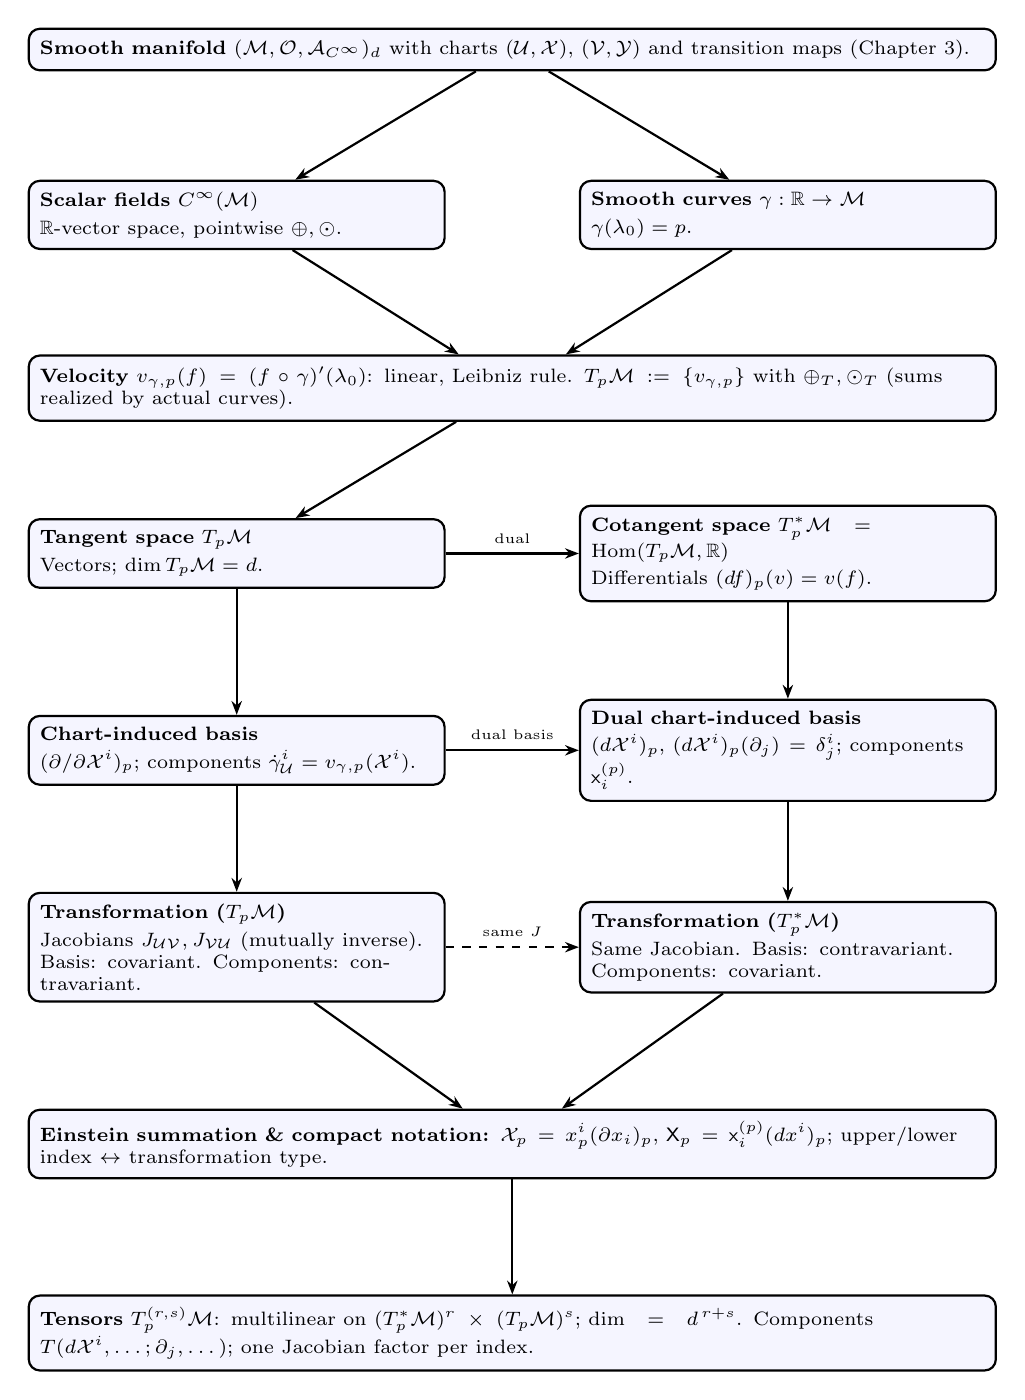
\begin{tikzpicture}[
  box/.style={draw, thick, rounded corners, fill=blue!4, align=left,
              text width=5.0cm, font=\scriptsize, inner sep=4pt},
  bigbox/.style={box, text width=12.0cm},
  aside/.style={box, fill=orange!5},
  ->, >={Stealth[length=5pt]}, thick
]

\node[bigbox] (root) at (3.5,0) {%
  \textbf{Smooth manifold $(\mathcal M,\mathcal O,\mathcal A_{C^\infty})_d$} with charts $(\mathcal U,\mathcal X)$,
  $(\mathcal V,\mathcal Y)$ and transition maps (Chapter 3).
};

\node[box] (sf) at (0,-2.1) {%
  \textbf{Scalar fields} $C^\infty(\mathcal M)$\\[2pt]
  $\mathbb R$-vector space, pointwise $\oplus,\odot$.
};
\node[box] (curve) at (7.0,-2.1) {%
  \textbf{Smooth curves} $\gamma:\mathbb R\to\mathcal M$\\[2pt]
  $\gamma(\lambda_0)=p$.
};

\node[bigbox] (vel) at (3.5,-4.3) {%
  \textbf{Velocity} $v_{\gamma,p}(f)=(f\circ\gamma)'(\lambda_0)$: linear, Leibniz rule.
  $T_p\mathcal M:=\{v_{\gamma,p}\}$ with $\oplus_T,\odot_T$ (sums realized by actual curves).
};

\node[box] (tp) at (0,-6.4) {%
  \textbf{Tangent space} $T_p\mathcal M$\\[2pt]
  Vectors; $\dim T_p\mathcal M=d$.
};
\node[box] (tsp) at (7.0,-6.4) {%
  \textbf{Cotangent space} $T^*_p\mathcal M=\mathrm{Hom}(T_p\mathcal M,\mathbb R)$\\[2pt]
  Differentials $(df)_p(v)=v(f)$.
};

\node[box] (bas) at (0,-8.9) {%
  \textbf{Chart-induced basis}\\[2pt]
  $(\partial/\partial\mathcal X^i)_p$; components $\dot\gamma^i_{\mathcal U}=v_{\gamma,p}(\mathcal X^i)$.
};
\node[box] (dbas) at (7.0,-8.9) {%
  \textbf{Dual chart-induced basis}\\[2pt]
  $(d\mathcal X^i)_p$, $(d\mathcal X^i)_p(\partial_j)=\delta^i_j$; components $\mathsf x_i^{(p)}$.
};

\node[box] (tr) at (0,-11.4) {%
  \textbf{Transformation ($T_p\mathcal M$)}\\[2pt]
  Jacobians $J_{\mathcal U\mathcal V},J_{\mathcal V\mathcal U}$ (mutually inverse).
  Basis: covariant. Components: contravariant.
};
\node[box] (dtr) at (7.0,-11.4) {%
  \textbf{Transformation ($T^*_p\mathcal M$)}\\[2pt]
  Same Jacobian. Basis: contravariant. Components: covariant.
};

\node[bigbox] (notn) at (3.5,-13.9) {%
  \textbf{Einstein summation \& compact notation:}
  $\mathcal X_p=x^i_p(\partial x_i)_p$, $\mathsf X_p=\mathsf x_i^{(p)}(dx^i)_p$; upper/lower index $\leftrightarrow$ transformation type.
};

\node[bigbox] (ten) at (3.5,-16.3) {%
  \textbf{Tensors} $T^{(r,s)}_p\mathcal M$: multilinear on $(T^*_p\mathcal M)^{r}\times(T_p\mathcal M)^{s}$;
  $\dim=d^{\,r+s}$. Components $T(d\mathcal X^{i},\dots;\partial_{j},\dots)$; one Jacobian factor per index.
};

\draw (root) -- (sf);
\draw (root) -- (curve);
\draw (sf) -- (vel);
\draw (curve) -- (vel);
\draw (vel) -- (tp);
\draw (tp) -- (tsp) node[midway, above, font=\tiny] {dual};
\draw (tp) -- (bas);
\draw (tsp) -- (dbas);
\draw (bas) -- (dbas) node[midway, above, font=\tiny] {dual basis};
\draw (bas) -- (tr);
\draw (dbas) -- (dtr);
\draw[dashed] (tr) -- (dtr) node[midway, above, font=\tiny] {same $J$};
\draw (tr) -- (notn);
\draw (dtr) -- (notn);
\draw (notn) -- (ten);

\end{tikzpicture}%
}
\end{center}

\end{document}
